%%
%% sample document for AAMAS'19 conference
%%
%% modified from sample-sigconf.tex
%%
%% see ACM instructions acmguide.pdf
%%
%% AAMAS-specific questions? F.A.Oliehoek@tudelft.nl
%%

\documentclass[sigconf]{aamas}  % do not change this line!

%% your usepackages here, for example:
\usepackage{booktabs}

\usepackage{amsthm}
\usepackage{amsmath,amssymb,amsfonts,xpatch}
\usepackage{algorithm}
\usepackage{algorithmic}
\newcommand{\expect}{\mathrm{Exp}}
\newcommand{\hide}[1]{}
%\newtheorem{theorem}{Theorem} % {\bfseries}{\itshape}
\newtheorem{observation}{Observation} % {\bfseries}{\itshape}
%\newtheorem{lemma}{Lemma}{\bfseries}{\itshape}
\newtheorem{problem}{Problem}
%\newtheorem{corollary}{Corollary}
\DeclareMathOperator*{\argmin}{arg\,min}
\newcommand{\opt}{\mathrm{OPT}}
\newcommand{\eopt}{E_{\mathrm{OPT}}}
\newcommand{\edeg}{e_{\mathrm{deg}}}
\newcommand{\prob}{\textsc{Spectral Radius Minimization}}
\newcommand{\numinf}{\#\text{inf}}
\newcommand{\kcsp}{k-\textsc{CSP}}
\newcommand{\kcrp}{k-\textsc{CRP}}
\newcommand{\infmax}{\textsc{IM}}
\newcommand{\wt}{\text{wt}}
\newcommand{\crit}{\text{crit}}
\newcommand{\loc}{\text{loc}}
\newcommand{\src}{\text{Src}}
%\newcommand{\avgcrit}{\text{AvgCrit}}
\newcommand{\avgcrit}{\text{ECrit}}
\newcommand{\maxcrit}{\text{MaxCrit}}
\newcommand{\algoavgcrit}{\textsc{ApproxECrit}}
\newcommand{\algomaxcrit}{\textsc{ApproxMaxCrit}}
\newcommand{\algosubmod}{\textsc{MaxSubmodConn}}
\newcommand{\algomaxst}{$k$-\textsc{MaxST}}
\newcommand{\greedy}{\textsc{Greedy}}
\newcommand{\R}{\mathcal{R}}
\newcommand{\HR}{H_{\R}}
\newcommand{\dist}{\texttt{dist}}
\newcommand{\ConnR}{\text{Conn}(\mathcal{R})}
\newcommand{\comp}{\text{comp}}
\newcommand{\degr}{\mathrm{d}}
\newcommand{\Vol}{\mathrm{Vol}}
\newcommand{\wmax}{w_{\max}}
\newcommand{\eps}{\epsilon}
\newcommand{\ceil}[1]{\left\lceil #1 \right\rceil}
\DeclareMathOperator*{\nodes}{nodes}
\DeclareMathOperator*{\walks}{walks}
\DeclareMathOperator*{\ct}{count}
\setlength{\abovedisplayskip}{3pt}
\setlength{\belowdisplayskip}{3pt}
\newcommand{\red}[1]{\textcolor{red}{#1}}



%% do not change the following lines
\usepackage{flushend}
\setcopyright{ifaamas}  % do not change this line!
\acmDOI{doi}  % do not change this line!
\acmISBN{}  % do not change this line!
\acmConference[AAMAS'20]{Proc.\@ of the 19th International Conference on Autonomous Agents and Multiagent Systems (AAMAS 2020), B.~An, N.~Yorke-Smith, A.~El~Fallah~Seghrouchni, G.~Sukthankar (eds.)}{May 2020}{Auckland, New Zealand}  % do not change this line!
\acmYear{2020}  % do not change this line!
\copyrightyear{2020}  % do not change this line!
\acmPrice{}  % do not change this line!

%% the rest of your preamble here


%%%%%%%%%%%%%%%%%%%%%%%%%%%%%%%%%%%%%%%%%%%%%%%%%%%%%%%%%%%%%%%%%%%%%%%%%%%%%%%%%%%%%%%%%%%%%%%%%%%%%%%%%

\begin{document}

\title{Finding Spatial Clusters Susceptible to Epidemic Outbreaks on a Social Contact Network}
%\title{Finding Spatial Clusters Susceptible to Epidemic Outbreaks due to Undervaccination}  % put your title here!
%\titlenote{Produces the permission block, and copyright information}

% AAMAS: as appropriate, uncomment one subtitle line; check the CFP
%\subtitle{Extended Abstract}
%\subtitle{Blue Sky Ideas Track}
%\subtitle{JAAMAS Track}
%\subtitle{Demonstration}
%\subtitle{Doctoral Consortium}

% AAMAS: submissions are anonymous for most tracks
\author{Paper \#1339}  % put your paper number here!

%% example of author block for camera ready version of accepted papers: don't use for anonymous submissions
%
%\author{Ben Trovato}
%\authornote{Dr.~Trovato insisted his name be first.}
%\orcid{1234-5678-9012}
%\affiliation{%
%  \institution{Institute for Clarity in Documentation}
%  \streetaddress{P.O. Box 1212}
%  \city{Dublin} 
%  \state{Ohio} 
%  \postcode{43017-6221}
%}
%\email{trovato@corporation.com}
%
%\author{G.K.M. Tobin}
%\authornote{The secretary disavows any knowledge of this author's actions.}
%\affiliation{%
%  \institution{Institute for Clarity in Documentation}
%  \streetaddress{P.O. Box 1212}
%  \city{Dublin} 
%  \state{Ohio} 
%  \postcode{43017-6221}
%}
%\email{webmaster@marysville-ohio.com}
%
%\author{Lars Th{\o}rv{\"a}ld}
%\authornote{This author is the
%  one who did all the really hard work.}
%\affiliation{%
%  \institution{The Th{\o}rv{\"a}ld Group}
%  \streetaddress{1 Th{\o}rv{\"a}ld Circle}
%  \city{Hekla} 
%  \country{Iceland}}
%\email{larst@affiliation.org}
%
%\author{Valerie B\'eranger}
%\affiliation{%
%  \institution{Inria Paris-Rocquencourt}
%  \city{Rocquencourt}
%  \country{France}
%}
%\author{Aparna Patel} 
%\affiliation{%
% \institution{Rajiv Gandhi University}
% \streetaddress{Rono-Hills}
% \city{Doimukh} 
% \state{Arunachal Pradesh}
% \country{India}}
%\author{Huifen Chan}
%\affiliation{%
%  \institution{Tsinghua University}
%  \streetaddress{30 Shuangqing Rd}
%  \city{Haidian Qu} 
%  \state{Beijing Shi}
%  \country{China}
%}
%
%\author{Charles Palmer}
%\affiliation{%
%  \institution{Palmer Research Laboratories}
%  \streetaddress{8600 Datapoint Drive}
%  \city{San Antonio}
%  \state{Texas} 
%  \postcode{78229}}
%\email{cpalmer@prl.com}
%
%\author{John Smith}
%\affiliation{\institution{The Th{\o}rv{\"a}ld Group}}
%\email{jsmith@affiliation.org}
%
%\author{Julius P.~Kumquat}
%\affiliation{\institution{The Kumquat Consortium}}
%\email{jpkumquat@consortium.net}
%
%% The example's default list of authors is too long for headers
%\renewcommand{\shortauthors}{B. Trovato et al.}


\begin{abstract}  % put your abstract here!
The standard public health intervention for controlling the spread of highly contagious
diseases like measles is vaccination at high rates.
However, in some states in the United States, even though the
average coverage is high, geographical clusters of undervaccinated
populations are emerging.
This raises the following fundamental questions: \emph{when do
undervaccinated clusters pose significant risk (i.e., become critical) for the
broader community?}  In particular, \emph{are all undervaccinated clusters
equally critical, or are some more critical than others?}
Given that public health resources are often limited, identifying and rank-ordering
critical clusters can help prioritize and allocate scarce resources for surveillance and
quick intervention.

We quantify the criticality of a cluster as the additional number of infections caused if
the cluster is underimmunized. This notion of criticality has not been studied before.
We focus on finding clusters that maximize this measure, and develop efficient approximation algorithms for finding critical clusters
by exploiting structural properties of the problem.
Finally, we apply our methods to the state of Minnesota, where we find clusters
with significantly higher criticality than those obtained by heuristics used in public health.
\end{abstract}


\keywords{AAMAS; ACM proceedings; \LaTeX; text tagging}  % put your semicolon-separated keywords here!

\maketitle


%%%%%%%%%%%%%%%%%%%%%%%%%%%%%%%%%%%%%%%%%%%%%%%%%%%%%%%%%%%%%%%%%%%%%%%%%%%%%%%%%%%%%%%%%%%%%%%%%%%%%%%%%
%% start of main body of paper

% !TEX root = ./main.tex
\section{Introduction}
Many highly contagious childhood diseases, such as measles, can be prevented by
vaccination. Therefore, it is worrisome that large outbreaks of such diseases 
have occurred in recent years, such as the measles
outbreaks in California in 2015 and in Minnesota in 2017---this is
despite high vaccination coverage in the US, e.g., $\sim 95\%$ for MMR, the measles vaccine. 
One of the reasons is the emergence of underimmunized geographical clusters, e.g., in California \cite{lieu2015geographic}
and Minnesota \cite{cadena:vacc-cluster}, often driven by misperceptions about 
side effects of vaccines \cite{atwell:pediatrics13}.  The typical response by public
health agencies is to monitor such clusters where immunization rates are falling, run active information campaigns, and engage community leaders. 

Cadena et al. \cite{cadena:vacc-cluster} use public school immunization data and identify six clusters in Minnesota,
which are statistically significant in terms of lower immunization rates, relative to the state wide level.
Implementing public health interventions in all these clusters is very expensive and time consuming for
public health agencies, which motivates the following problem: \textbf{\emph{which of these clusters (which are very different
in terms of size, immunization rates, and demographics) pose the most risk, and should be prioritized for response.}}
This is supported by Metcalf et al.~\cite{metcalf:epidemics15},
who state that \emph{``[t]here is also a need to understand under what conditions such clusters become at 
risk for epidemic spread, and the risk they pose to surrounding groups where vaccine coverage may be high.''} 
Since immunization rates are falling, it is useful to consider not only clusters in which these rates
are presently low, but also the clusters which would pose a risk if fewer people within them got vaccinated.
We develop a method to address these important public health policy questions.
Our contributions are summarized below.
\smallskip




\begin{figure}
\centering
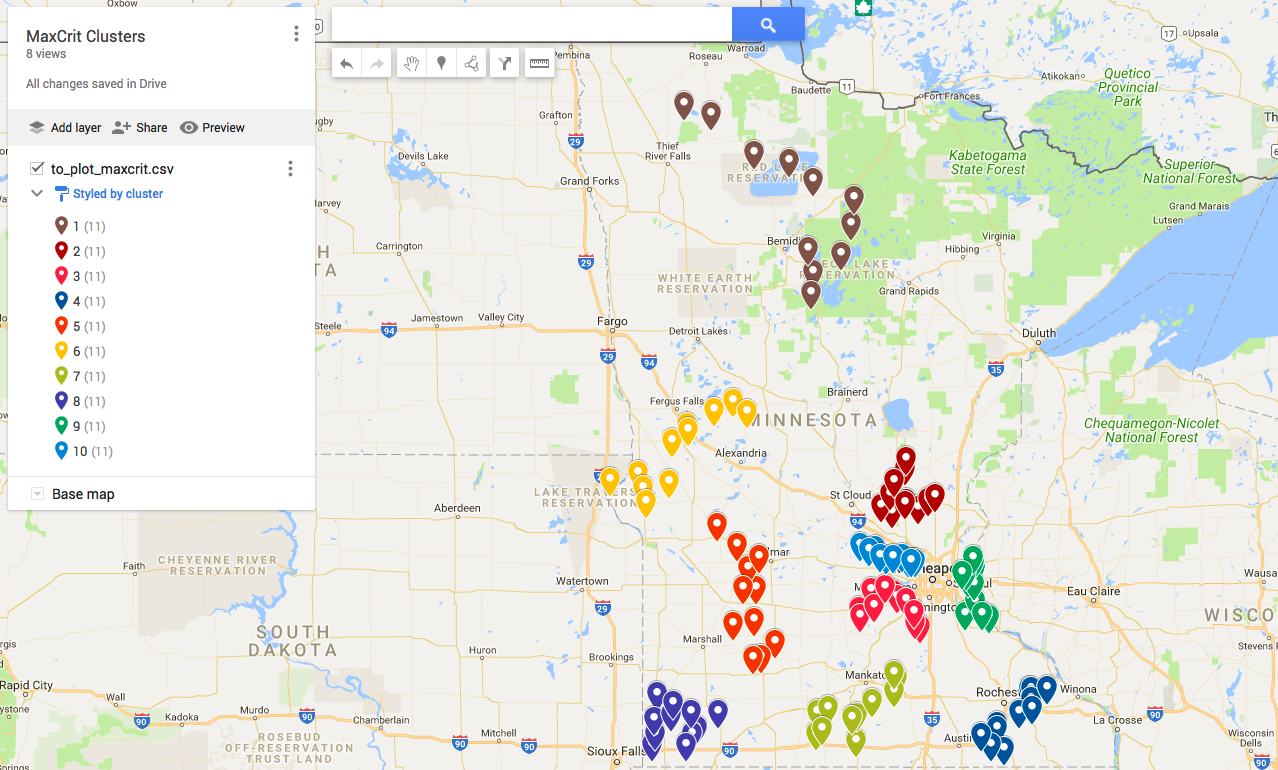
\includegraphics[width=.45\textwidth]{img/maxcrit_clusters.png}
\caption{Critical sets in Minnesota discovered using our methods. These are contiguous regions that lead to large measles outbreaks if not properly vaccinated.
\vspace*{-0.15in}
}
\label{fig:mn-criticalsets}
\end{figure}
%
%\begin{enumerate}
%\item 
\noindent
\textbf{1. Formalizing critical clusters.}
We formalize the notion of \emph{criticality} in a population represented as a social contact network $G=(V, E)$, with a spatial embedding $\HR$ (defined later). The criticality of a subset $S$ of the population is defined as the \emph{expected number of additional infections} that would occur if the immunization rate within $S$ is low. We are interested in clusters $S$ that (1) are contiguous in space, with respect to the spatial embedding network $\HR$ and (2) have the maximum criticality. We refer to this optimization task as the $\maxcrit{}$ problem. 

The spatial proximity is motivated by a public health response perspective, as in \cite{lieu2015geographic,atwell:pediatrics13,cadena:vacc-cluster}. Public health interventions involve intensive field work, and these interventions are most effective within a small region. This motivates the problem of finding a contiguous spatial cluster of bounded size with maximum criticality,
which are the kinds of clusters reported in \cite{cadena:vacc-cluster}.

%We formalize the notion of criticality in a social contact network $G=(V, E)$, which is associated with a spatial embedding, represented as a graph $\HR$ (defined formally later). The criticality of a subset $S$ is defined as the \emph{expected number of additional infections} that would occur if the immunization rate within $S$ is low. We are interested in clusters $S$ that 1) are contiguous in space and 2) have the maximum criticality---this is referred to as the \maxcrit{} problem. The spatial proximity is motivated by a public health response perspective, as in \cite{lieu2015geographic,atwell:pediatrics13}. Public health interventions involve intensive field work, which is another motivation for clusters corresponding to contiguous regions. Further, such response is most effective within a small region. This motivates the problem of finding a contiguous spatial cluster $S$ of bounded size with maximum criticality. Our contributions are as follows.


\noindent
\textbf{2. Rigorous algorithms for $\maxcrit{}$.}
The $\maxcrit{}$ problem is computationally very challenging. We show that \maxcrit{} is NP-hard and design algorithm \algomaxcrit{}, which has a worst case approximation guarantee of $\Omega(1/k^{(d-1)/(2d-1)})$, relative to the optimum, for clusters of size $k$. Here, $d$ is related to the complexity of the spatial embedding network $\HR$, and it is a constant in practice. 

We also show that the criticality function is submodular, which implies that $\maxcrit{}$ is equivalent to the classical Influence Maximization (\infmax) problem \cite{kempe:sigkdd03}, \emph{with an important constraint that the seed set is connected}. Due to this connectivity requirement, the standard greedy algorithms for \infmax{} yield poor results. %We also improve the running time significantly using a careful sampling technique.
A corollary of our results is an $\Omega(1/k^{(d-1)/(2d-1)})$ approximation for maximizing any non-negative monotone submodular function over the set of connected subgraphs of size $k$ in a graph with doubling dimension $d$. For any $d\geq0$, we have $1/k^{(d-1)/(2d-1)}\geq 1/\sqrt{k}$, so our result improves the previous best $\Omega(1/\sqrt{k})$-approximation for submodular maximization with connectivity constraints \cite{kuo2015maximizing}.

%Here, $d$ denotes the \emph{doubling dimension} of the associated spatial graph $\HR$ (defined later), and is a constant in practice, e.g., $2$ for a grid. We show that the \maxcrit{} objective is submodular, and this problem is equivalent to the classical Influence Maximization (\infmax) problem

%\item
\noindent
\textbf{3. Application.} 
We evaluate our algorithm on a detailed population and contact network model for the state of Minnesota.
The sets we discover have very high criticality compared to
heuristics commonly considered for public health interventions.
We achieve over 25\% higher criticality for the objective compared to all the baselines.
The critical clusters discovered using our algorithms (shown in Figure \ref{fig:mn-criticalsets})
have meaningful demographic properties
from a public health perspective: they typically involve people with lower than average
income and age (Section \ref{sec:experiments-cs}).
We also compute the criticalities of the clusters reported in \cite{cadena:vacc-cluster}.
Quite surprisingly, we find that: (1) the cluster with lowest vaccination rate among these is not the most critical, and
(2) the cluster computed using our algorithm has criticality more than 10 times that of any of the clusters
identified by \cite{cadena:vacc-cluster}.


Finally, because of the lack of public outbreak data, there is no easy way to validate our results, but we note that \emph{one of the clusters we found to be critical lies in the Minneapolis metropolitan area where a large measles outbreak occurred in 2017 \cite{hall:mmwr17}}.


\noindent
\textbf{Social impact.}
Our method for finding critical sets, applied to detailed population and contact network models (which are now standard approach in public health), provides an operational tool for public health agencies in prioritizing their limited surveillance and public outreach resources.
Our results imply that from a public health perspective, it is important to address not just the current undervaccinated clusters
identified in \cite{cadena:vacc-cluster}, but also make sure that the immunization rates in the critical clusters does not fall.







% !TEX root = ./main.tex
\section{Preliminaries}
\label{sec:background}
\begin{figure}
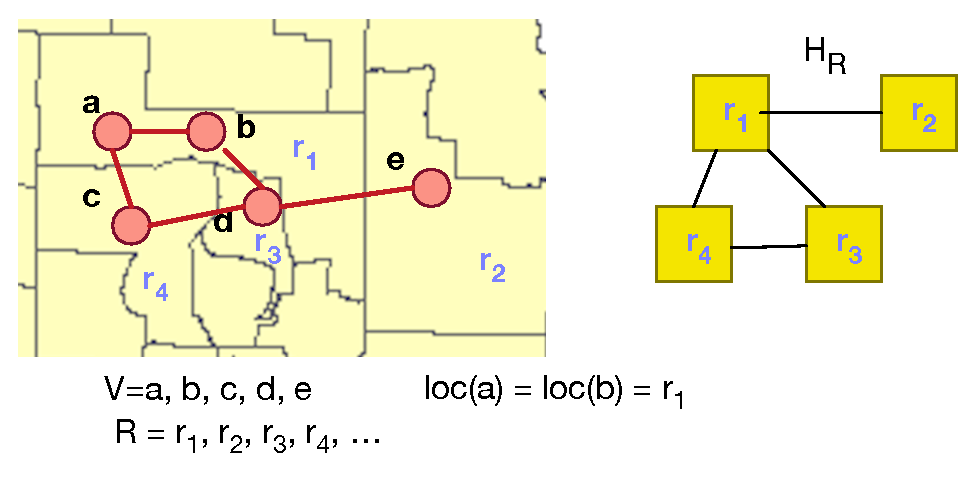
\includegraphics[width=0.45\textwidth]{img/example.pdf}
\vspace{-.2in}
\caption{Notation used in the paper. The 5 red circle nodes $(a,b,c,d,e)$ form a social contact network. Each node resides in a block group $r_i$, and these block groups form the block group graph $H_\mathcal{R}$, where an edge represents that the block groups are adjacent on the map.}
\label{fig:definitions-example}
\end{figure}
\subsection{Disease spread on a social contact network}
Let $V$ denote a population, and let $G=(V, E)$ be a contact graph on which a disease can spread. A person or node $v \in V$ can propagate the disease to its neighbors. There is an edge between two people if they come into close proximity during a typical day. For example, the nodes represent two coworkers in the same building, students in the same classroom, or members of the same household. 
Additionally, %in the social contact network datasets that we consider (Section \ref{sec:data}),
each person $v$ is associated with a geographical location---i.e., their place of residence---denoted by $\loc(v)$;
we will consider such locations at the resolution of census block groups.
Let $\mathcal{R}$ denote the geographical area where the nodes $V$ are located---for example, the state of Minnesota---and let $\mathcal{R}=\{r_1,\ldots,r_N\}$ be a decomposition of $\mathcal{R}$ into
census block groups. For a block group $r_i\in\mathcal{R}$, we use $V(r_i)$ to denote the
set of nodes associated with location $r_i$; that is, those with $\loc(v)\in r_i$. Analogously, for a set of block groups or \emph{region} $R\subset \R$, let $V(R)=\cup_{r_i\in R} V(r_i)$ be the set of nodes located within $R$. We consider a graph $H_{\R}=(\R, E_{\R})$ on the set of block groups, where
two block groups are connected if they are geographically contiguous, i.e., they are adjacent on a map. In particular, we are interested in \emph{connected} subgraphs of $H_{\R}$. We use $\ConnR$ to denote all the subsets $R\subset \HR$ that are spatially connected. These definitions are illustrated in Figure \ref{fig:definitions-example}.
%$(R_i, R_j)\in E_{\R}$ if $R_i$ and $R_j$ have a common boundary.
%Let $\ConnR$ denote subsets $R\subset \HR$ that are spatially connected in the block group graph $H_{\R}$.

\begin{table}[ht]
\begin{footnotesize}
\centering \caption{
Summary of the notation used in the paper
}
\label{table:notation}
\begin{tabular}{|p{0.9in}|p{2.2in}|}
\hline
\textbf{Notation} & \textbf{Description} \\
\hline
$G=(V, E)$ & Contact graph on set $V$ of individuals\\
$\loc(v)$ & Geographical location of node $v$\\
$\mathcal{R}=\{r_1,\ldots,r_N\}$ & Entire geographical area where the nodes $V$ are located---e.g., Minnesota partitioned into block groups $r_i$\\
$V(r_i)$ & Set of nodes of $G$ with $\loc(v)=r_i$\\
$V(R)$ & $\cup_{r_i\in R} V(r_i)$\\
$H_{\R}=(\R, E_{\R})$ & Network on $\R$, with adjacent block groups connected by an edge.
Sometimes referred to as ``the auxiliary network.''\\
$\ConnR$ & Set $R\subset \R$  spatially connected in $H_{\R}$\\
%S, E, I, R & States in the disease model\\
$\gamma$ & Average region-wide vaccination rate\\
$\mathbf{x}$ & Vaccination vector, with $x_i$ denoting the probability that node $i$
is vaccinated\\
$\mathbf{x}^R$ & Vaccination vector, with nodes $V(R)$ undervaccinated, where $R\in\ConnR$\\
$\src_A$, $\src$ & Denotes the event that the  infection source is from a 
set $A\subset \R$. $\src$ is used when $A=\R$ \\
$\numinf(\mathbf{x}, \src_A)$ & Expected number of infections for
vaccination vector $\mathbf{x}$ and source being $\src_A$\\
%$\crit(R, \mathbf{x}, \src_A)$ & Criticality of $R$: expected number of additional infections if $R$ is not vaccinated\\
$\maxcrit(R)$, $\maxcrit(R, \mathbf{x})$ & The objective value of $\maxcrit{}$ for region
$R\in\ConnR$ in an instance $(G, H_{\R}, k)$\\
%$\avgcrit(R)$, $\avgcrit(R, \mathbf{x})$ & The objective value of $\avgcrit{}$ for region
%$R\in\ConnR$ in an instance $(G, H_{\R}, k)$\\
\hline
\end{tabular}
\end{footnotesize}
\end{table}

\noindent
\textbf{Distances and geometry of $\HR$.}
For $u, v\in \R$, let $\dist_{\HR}(u, v)$ denote the distance between $u$ and $v$ in the graph $\HR$, which is equal to the length of the shortest path between them.
The ball centered at $v$, with radius $\ell$ is defined as $B_{\HR}(v, \ell)=\{u: \dist(u, v)\leq\ell\}$, which is the set of all nodes within distance $\ell$ of $v$. When the graph is clear from the context, we drop it from the subscript in the notation for $B(\cdot)$ and $\dist(\cdot)$.
We say that the graph $\HR$ has \emph{doubling dimension} $d$ if it satisfies the following property: any ball $B(v, \ell)$ can be covered by at most $2^d$ balls of radius $\ell/2$ \cite{gupta:focs03}. Geometric graphs, such as grids, have constant doubling dimension, usually around $2$; note that $d$ need not be an integer. Our approximation guarantees will be in terms of $d$.

\noindent
\textbf{Disease model.} We use an SEIR model for diseases like measles \cite{anderson+m:book}, 
where a node is in one of four states:
Susceptible (S), Exposed (E), Infected (I), and Recovered/Removed (R). Measles is highly contagious, and an infected node spreads the
disease to each susceptible neighbor with high probability. 
Sometimes, we assume a transmission probability of 1, but our results
extend to the more general case. If a node is vaccinated,
it does not get infected. We assume the vaccine has 100\% efficacy, which is
not true in practice, but this is not crucial for our methodology.

Let $\gamma$ denote the average region-wide vaccination rate---around $0.97$
in Minnesota. Let $\mathbf{x}$ be a \emph{vaccination} or \emph{intervention} vector: 
$x_i\in[0,1]$ denotes the probability that node $i$ is vaccinated (so $x_i=\gamma$,
by default).
Let $\src_A$ denote the source of the infection or \emph{initial conditions} of the disease process: this could be one or a small number of nodes from a region $A\subset \mathcal{R}$, which initially get infected. We use $\numinf(\mathbf{x}, \src_A)$ to denote the expected number of infections
given an intervention $\mathbf{x}$ and initial conditions $\src_A$.
When $\src_A$ is clear from the context, we simply use $\numinf(\mathbf{x})$.
  
%\subsection{Criticality and Problem Formulation}
\subsection{Criticality}
For a vaccination vector $\mathbf{x}$,
let $\mathbf{x}^S$ denote the corresponding intervention where a subset $S\subset V$ of
nodes is undervaccinated. That is,
$\mathbf{x}^S_i = \mathbf{x}_i$ for $i\not\in S$ and $\mathbf{x}^S_i=\gamma'$ for $i\in S$,
where $\gamma'$ is much lower than $\gamma$, the region-wide vaccination rate.
Without loss of generality, we sometimes consider $\gamma'=0$ for mathematical convenience.

\setlength{\abovedisplayskip}{3pt}
\setlength{\belowdisplayskip}{3pt}

%We define the \textbf{criticality} of a set $S\subset V$ as
%$\crit(S, \mathbf{x}, \src_A) = \numinf(\mathbf{x}^S, \src_A) - \numinf(\mathbf{x}, \src_A)$,
%which is the \emph{expected number of additional infections that occur if $S$ is not vaccinated}
%(with respect to any specific initial conditions $\src_A$).
%Our focus is on finding spatial clusters of high criticality, so %Therefore, the set $S$
%of nodes in the above notion of criticality must be located in a connected geographical region.
%we focus on $S=V(R)$ for a connected region $R\in\ConnR$.

We define the \textbf{criticality} of a set $S\subset V$ as
the \emph{expected number of additional infections that occur if $S$ is not vaccinated},
with respect to some initial condition $\src_A$.
Because we are interested on finding spatial clusters of high criticality, 
we focus on $S=V(R)$ for a connected region $R\in\ConnR$.
Then, we define the criticality of a region as
\[
\crit(R, \mathbf{x}, \src_A) = \numinf(\mathbf{x}^R, \src_A) - \numinf(\mathbf{x}, \src_A),
\]
which is the expected number of extra infections if nodes in the region $R$ are undervaccinated. In order to simplify the notation, we will drop $\mathbf{x}$ and $\src$ from the inputs to $\crit(\cdot)$, whenever it is clear from the context.


%Then, we pose the task of finding spatial clusters of high criticality as the following optimization problem.

\section{Problem Formulation}
\label{sec:problem-statement}

\noindent 
\texbf{Modeling considerations.} In practice, public health interventions involve intensive field work---e.g., targeted information campaigns. Furthermore, these interventions are most effective within small, localized geographical regions. Therefore, we focus on finding regions that have high criticality \emph{and} small size. In modeling terms, this can be accomplished by adding a size parameter $k$, which can be tuned based on the available public health resources. 

Given the discussion above, we pose the task of finding spatial clusters of high criticality as the following optimization problem.
\begin{problem}[$\maxcrit{}(G, H_{\R}, k)$]
\label{prob:maxcrit}
Given an instance $(G, H_{\R}, k)$, find a connected region $R\in\ConnR$ of size at most $k$ that maximizes criticality over all choices of source:
\[
R= \mbox{\emph{argmax}}_{R'\in\ConnR, |R'|\leq k} \text{\emph{crit}}(R', \mathbf{x}, \src_{R'})
\]
\end{problem}

In words, the $\maxcrit{}$ problem involves maximizing over \emph{all} possible
choices of the sources $\src_{R'}$ in the cluster $R'$. We emphasize that the disease spreads on the social network $G$ of \emph{individuals}, whereas the connectivity constraint is imposed on the graph $\HR$ of \emph{census block groups}, since we're interested in finding a spatial cluster. From a public health perspective, our problem models the following question: \emph{what is the most critical cluster of size $k$ if the disease starts within the undervaccinated cluster itself?} An obvious question is how should the parameter $k$ be chosen. As mentioned earlier, this can depend on the resources of the public health department, since interventions are very localized.

% This is formalized as
%We use $\maxcrit(R, \mathbf{x}, \src)$ or 
%$\maxcrit(R)$ to denote the objective value of an instance of the problem.


% $\max_{\src_R} \crit(R, \mathbf{x}, \src_R)$, the objective value of $\maxcrit{}$ for region $R$ in an instance $(G, H_{\R}, k)$.



%\subsection{Submodularity}
%A set function $f: 2^V \rightarrow \mathbb{R}$ is said to be \emph{submodular} if it satisfies the diminishing returns property: for any $T \subset S\subset V$ and $x \in V\setminus S$, we have that
%$$
%f(T \cup x) - f(T) \geq f(S \cup x) - f(S).
%$$
%That is, the marginal gain of adding $x$ to a set is larger on a smaller context. 
%
%Submodularity has become popular in recent years in machine learning \cite{krause2008beyond} because 1) the diminishing returns property applies naturally to many problems of interest (e.g., sensor placement) and 2) there exist simple algorithms for approximate constrained submodularity maximization \cite{nemhauser1978analysis}---though the problem is NP-Hard in general. For the problem of maximizing a submodular function over subsets of size at most $k$, Nemhauser et al.\ \cite{nemhauser1978analysis} proposes the following greedy algorithm. We start with the empty set $S_0 = \emptyset$. We construct a set $S_i$ by adding an element to $S_{i-1}$ that yields the highest increase in objective value:
%$$
%S_{i} = S_{i - 1} \cup \operatornamewithlimits{argmax}_{x \in V \setminus S_{i - 1}} \{f(S_{i - 1} \cup \{x\}) - f(S_{i - 1})\}
%$$
%The algorithm returns a set $S_k$ as the solution, with objective value at least $1 - \frac{1}{e}$ of the optimal. We refer to this procedure as \emph{the greedy algorithm}.
%
%We focus on submodular function maximization with connectivity constraints.
%\begin{problem}
%\label{prob:connected-submodular}
%Given a graph $G=(V,E)$, a non-negative submodular function $f: 2^V \rightarrow \mathbb{R}^+$, and a parameter $k$, the objective is to find a set $S\subset V$ of size at most $k$ that maximizes $f$.
%\end{problem}
%
%As we discuss in Section \ref{sec:proposed-critical}, the \kcsp{} and \kcrp{} problems are equivalent to Problem \ref{prob:connected-submodular}.
%
%
%\subsection{Notes on problem formulations}
%
%Extending the earlier definitions to take initial conditions into account.
%\begin{itemize}
%\item
%Let $\mathbf{s}$ be a distribution specifying the source. 
%\item
%Let $Src_A$ denote the event that the source is in set $A$ of block groups. Let
%$p(Src_A)$ denote the probability of this event; it is proportional to the number of
%block groups in $A$
%\item
%$\numinf(\mathbf{x}, \mathbf{s})$ is the expected number of infections that occur
%when the intervention vector is $\mathbf{x}$ and the source is distributed according to
%the distribution $\mathbf{s}$. 
%\item
%$\numinf(\mathbf{x}, Src_A)$ is the expected number of infections that occur, conditioned
%on the event $Src_A$ occurring, i.e., if the source is uniformly distributed in $A$
%\item
%$\avgcrit(S, \mathbf{x}, \mathbf{s}) = \numinf(\mathbf{x}^S, \mathbf{s}) - 
%\numinf(\mathbf{x}, \mathbf{s})$ is the criticality of $S$, 
%where $\mathbf{s}$ denotes a set of sources.
%\item
%$\maxcrit(S, \mathbf{x}) = \max_{\mathbf{s}} \numinf(\mathbf{x}^S, \mathbf{s}) - 
%\numinf(\mathbf{x}, \mathbf{s})$ is the criticality of $S$, over all possible source distributions.
%In practice, $\maxcrit(S)$ will be maximized for an event $Src_S$, i.e., when the source
%is actually in $S$.
%\item
%Problem 1: critical set when the source is distributed independently. 
%Given a set $\mathbf{s}$ of sources, this is formalized as the following problem
%\[
%\mbox{argmax}_{R', |R'|\leq k} \avgcrit(R', \mathbf{x}, \mathbf{s})
%\]
%\item
%Problem 2: critical set when the source is chosen to be one that maximizes the criticality.
%This is formalized as the following problem
%\[
%\mbox{argmax}_{|R'|\leq k} \maxcrit(R', \mathbf{x})
%\]
%\end{itemize}
%
%Some observations
%\begin{itemize}
%\item
%For any monotone function $F(\cdot)$ and disjoint sets $A_1, A_2$,
%we have $F(A_1\cup A_2) \geq \frac{1}{2}F(A_1) + \frac{1}{2}F(A_2)$. This follows from the
%following reason: suppose $F(A_1)\geq F(A_2)$. Then, by monotonicity, we have
%\[
%F(A_1\cup A_2)\geq F(A_1)\geq \frac{1}{2}F(A_1) + \frac{1}{2}F(A_1) \geq \frac{1}{2}F(A_1) + \frac{1}{2}F(A_2) 
%\]
%Such a property does not imply $(r, \gamma)$-locality in \cite{krause2006near}, because
%they need the following property: for disjoint sets $A_1, A_2,\ldots, A_k$
%\[
%F(A_1\cup A_2\cup\ldots A_k)\geq \gamma\sum_{i=1}^k F(A_i)
%\]
%If the stronger property of $(r, \gamma)$-locality from \cite{krause2006near} holds, then
%the above property follows because
%\begin{eqnarray*}
%F(A_1\cup A_2\cup\ldots A_k) &\geq& F(A_1\cup A_2\cup\ldots A_{k-1}) + \gamma F(A_k)\\
%&\geq& F(A_1\cup A_2\cup\ldots A_{k-2}) + \gamma F(A_{k-1}) + \gamma F(A_k)\\
%&\geq& \ldots
%\end{eqnarray*}
%\item
%The objective $\maxcrit(\cdot)$ is not $(r,\gamma)$ local. Consider a setting
%where each block group induces a clique, which is disjoint from all other block groups.
%Then, $\maxcrit(A_1)\propto \max_{b\in A_1} |V(b)|$ is proportional to the largest
%block group in the set $A_1$. Similarly, we have $\maxcrit(A_2)\propto \max_{b\in A_2} |V(b)|$.
%For disjoint sets $A_1, A_2$, we have
%\[
%\maxcrit(A_1\cup A_2) = \max_{b\in A_1\cup A_2} |V(b)| < \maxcrit(A_1) + \maxcrit(A_2)
%\]
%\item
%The solutions are different for these formulations can be different. 
%Suppose a graph has is a large 
%Solutions that optimize
%$\maxcrit(\cdot)$ will be large clusters, which are s
%\end{itemize}
%
%\comment{somewhere: put justification for both problems and using synthetic populations}


% !TEX root = ./main.tex
%\section{Key properties of criticality}
%\label{sec:structure}
%We describe connections
%between the proposed problems and Influence
%Maximization, which will have implications on the computational complexity.
%We also prove structural properties of these objectives, later used in our algorithms.


\section{Computational challenges}

\subsection{Hardness of $k$-\maxcrit{}}

\begin{theorem}
\label{theorem:nphard}
\emph{MaxCrit} is NP-hard.
\end{theorem}

We present the proof in the Supplementary Material. The main idea is to show that \maxcrit{} is equivalent to
the classical Influence Maximization (\infmax) problem \cite{kempe:sigkdd03}. Briefly, in \infmax, we are given a directed graph, disease transmission probabilities for each edge, and a size constraint $k$. The goal is to find a \emph{seed set} of $k$ nodes to be the source of an infection, such that the number of infected nodes, following a given disease model, is maximized. 
While \maxcrit{} has a different objective, we show that it can be viewed as \infmax{} not on $G$ but as an expectation on
different graph in which all vaccinated nodes are removed with the corresponding probability,
and a meta-node is added to ensure connectivity.


\subsection{Poor performance of \infmax{} solutions}

Though \maxcrit{} is closely related to \infmax, we cannot directly apply the current methods for 
\infmax{}. This is because the connectivity constraint has a strong effect on the solution of \maxcrit{}. A solution computed for \infmax{} using the greedy algorithm of \cite{kempe:sigkdd03} can be arbitrarily suboptimal for \maxcrit{}. Informally, this follows because, in \infmax{}, it is better to choose seeds that are far apart and disconnected, so that their combined number of infections is maximized.

\begin{observation}
\label{obs:infmax}
There exists a family of instances $(G, H_{\R}, k)$ for which the optimum solution
$S^*$ to \maxcrit{} satisfies
$\maxcrit(S^*) =O(\frac{1}{k}\infmax(\hat{S}))$, where $\hat{S}$ is the optimum
solution to the \infmax{} version for this instance, without any connectivity requirements.
\end{observation}

For example, consider a cycle graph, as in Figure \ref{fig:observation}. Every node has one outgoing neighbor (clockwise direction), and every node infects its neighbor with probability 1, unless the neighbor is a blue node, in which case the probability is 0, as denoted in the figure. There are $k=4$ spreader nodes (in blue) separated by paths of length $k+1$. Consider an instance of $\infmax{}$ with size constraint $k$, and the analogous instance of $\maxcrit{}$, where, for simplicity, we assume that $G = \HR$. The optimal solution to \infmax{} consists of the $k$ hub nodes, with objective value equals to the number of nodes in the graph, $k(k+1)$, since each hub is able to propagate the infection through all the white nodes until the next clockwise hub. In contrast, the solution to \maxcrit{} must be a connected set of nodes, so the best solution would consist of a hub and the next $k$ clockwise white nodes, for an objective value of $k + 1$.

\begin{figure}
    \centering
    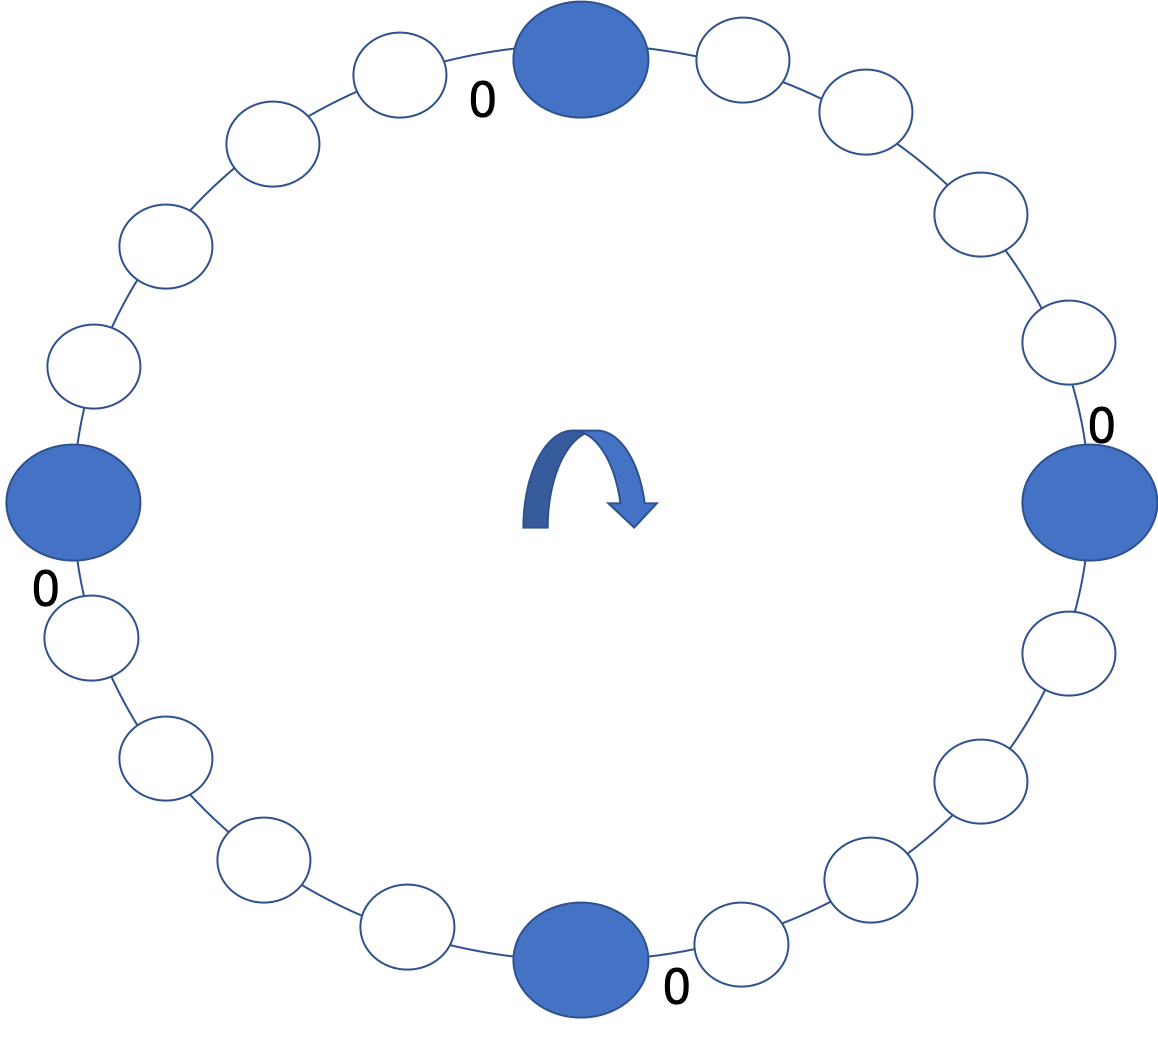
\includegraphics[width=.5\columnwidth]{img/observation.png}
    \caption{Effect of connectivity constraint in cycle graph with $k=4$ spreader nodes (blue) separated by paths of length $k + 1$. The optimal solution to $\infmax{}$ has $k$ times the objective value of the optimal solution for \maxcrit{}. See text for details.}
    \label{fig:observation}
\end{figure}

%\subsection{Submodularity of \maxcrit{} and \avgcrit{}}
%\label{sec:submodular}
%A set function $f: 2^V \rightarrow \mathbb{R}$ is said to be \emph{submodular} if it satisfies the diminishing returns property: for any $T \subset S\subset V$ and $x \in V\setminus S$, we have that $f(T \cup \{x\}) - f(T) \geq f(S \cup \{x\}) - f(S)$. In recent years, there has been notable interest in submodularity as a key property to approach problems in machine learning. We exploit this property to design efficient algorithms for the proposed problems.%We have the following result:
%
%\begin{lemma}
%\label{lemma:submodular}
%$\maxcrit{}$ and $\avgcrit{}$ are submodular.
%\end{lemma}

%\begin{proof}
%Consider a random live graph $L(V, E')$ defined as above, and let $\crit_{L}(S, \mathbf{x})$ be the criticality of $S\subset V$ on this graph. Without loss of generality, assume there is only one initial infection and let $r$ be the initially infected node. Then, the criticality of $S$ can be computed as
%$$
%\crit_L(S, \mathbf{x}) = |\left(\bigcup_{s \in S} \text{comp}_L(s)\right) \cup \text{comp}_L(r)| - |\text{comp}_L(r)|.
%$$
%In words, the number of extra infections in $L$ due to node set $S$ is the size of the union of the components of nodes in $S$ minus the infections that we get if only the seed is infected---i.e., the size of $\text{comp}_L(r)$.
%
%Now, consider two sets $S,T$, such that $T\subseteq S$, and a node $v \not \in S$. The quantity $\crit_L(T \cup \{v\}, \mathbf{x}) - \crit_L(T, \mathbf{x})$ is the number of extra infections from adding node $v$; that is, the number of elements in $\text{comp}_L(v)$ that are not already in $(\bigcup_{s \in T} \text{comp}_L(s)) \cup \text{comp}_L(r)$. This number is at least as large as the number of extra infections that we get by adding $v$ to the bigger set $S$, which gives us $\crit_L(T \cup \{v\}, \mathbf{x}) - \crit_L(T, \mathbf{x}) \geq \crit_L(S \cup \{v\}, \mathbf{x}) - \crit_L(S, \mathbf{x})$. This is precisely the definition of submodularity, so the criticality function for a fixed graph is submodular. Over random realizations of $L$, we obtain
%$$
%\crit(S, \mathbf{x}) = \sum_{L}\text{Pr}(L) \crit_L(S, \mathbf{x}).
%$$
%This is a convex combination of submodular functions, which is known to be submodular too, completing the proof.
%\end{proof}

%We present the proof in the Supplementary Material. The argument is similar to the submodularity proof for \infmax{}.

\section{Proposed Methods}
\label{sec:proposed-critical}
Our strategy involves showing that the $\crit$ function is submodular; then, the $\maxcrit{}$ problem reduces to maximizing a submodular function over connected subgraphs of $\HR$. We start with the necessary definitions.

\subsection{Submodular function maximization with connectivity constraints}
\label{sec:submod-connectivity}
A set function $f: 2^{\R} \rightarrow \mathbb{R}$ is said to be \emph{submodular} if it satisfies the diminishing returns property: for any $S \subset S'\subset \R$ and $x \in \R\setminus S'$, we have that $f(S \cup \{x\}) - f(S) \geq f(S' \cup \{x\}) - f(S')$. That is, we obtain a larger increase in $f$ when adding an element $x$ to a smaller set. In recent years, there has been notable interest in submodularity as a key property to approach problems in machine learning \cite{krause2008beyond}. 

Here, we consider $f(S)=\crit(S, \mathbf{x}, \src)$. For notational simplicity, we will drop $\mathbf{x}$ and $\src$. Our first key result is that $\crit$ is submodular. %(proof in the Supplementary Material).

\begin{lemma}
$\text{\emph{\crit(}S\text{\emph{)}}}$ is a submodular function of $S\subset\R$.
\end{lemma}

\begin{proof}
We follow the approach of Kempe et al.\ \cite{kempe:sigkdd03}, who analyze one random realization of the diffusion process at a time. For simplicity, we prove the submodularity of $\crit$ for the Independent Cascade model, but the result extends to the more general SEIR process. For each edge $e=(u,v)$, we flip a coin with bias equal to the transmission probability $p(u,v)$. Let $X(e)$ be a Bernoulli variable that is 1 with probability $p(u,v)$; then, we define the \emph{live} graph $L(V, E')$ as the subgraph of $G$ induced by the edges for which $X(e) = 1$: $L' = (V, E'=\{e \in E | X(e) = 1\})$. In the live graph, a node $v$ is infected by the end of the diffusion process if and only if $v$ is in the same component as one of the seeds in $S$. Without loss of generality, assume there is only one initial infection and let $r$ be the initially infected node. Then, the criticality of $S$ can be computed as
$$
\crit_L(S) = \left|\left(\bigcup_{s \in S} \text{comp}_L(s)\right) \cup \text{comp}_L(r)\right| - \left|\text{comp}_L(r)\right|.
$$
In words, the number of extra infections in $L$ due to node set $S$ is the size of the union of the components of nodes in $S$ minus the infections that we get if only $r$ is infected---i.e., the size of $\text{comp}_L(r)$.

Now, consider two sets $S,T$, such that $T\subseteq S$, and a node $v \not \in S$. The quantity $\crit_L(T \cup \{v\}) - \crit_L(T)$ is the number of extra infections from adding node $v$; that is, the number of elements in $\text{comp}_L(v)$ that are not already in $(\bigcup_{s \in T} \text{comp}_L(s)) \cup \text{comp}_L(r)$. This number is at least as large as the number of extra infections that we get by adding $v$ to the bigger set $S$, which gives us $\crit_L(T \cup \{v\}) - \crit_L(T) \geq \crit_L(S \cup \{v\}) - \crit_L(S)$. This is precisely the definition of submodularity, so the criticality function for a fixed live graph is submodular. Over random realizations of $L$, we obtain
$$
\crit(S) = \sum_{L}\text{Pr}(L) \crit_L(S).
$$
where $\text{Pr}(L)$ denotes the probability of obtaining the live graph $L$ with the edge probabilities $p(u,v)$. This is a convex combination of submodular functions, which is known to be submodular too, completing the proof.
\end{proof}

The \maxcrit{} problem can be seen as maximizing the submodular function $\crit(S)$ over all connected $S\in\ConnR$, with $|S|\leq k$. The connectivity constraint significantly increases the computational complexity of the problem. In contrast, the relaxed problem of maximizing a submodular function subject \emph{only} to a size constraint $k$ can be approximated to a constant factor. Given a submodular function $f(\cdot)$, the $\greedy{}$ algorithm of \cite{nemhauser1978analysis} finds a set $S$ with objective value at least $(1 - 1/e)$ of the optimal by iteratively adding a node $v$ to $S$ that maximizes the marginal benefit, $f(S\cup\{v\}) - f(S)$.
For submodular maximization with connectivity constraints, \cite{kuo2015maximizing} give an $\Omega(1/\sqrt{k})$ approximation guarantee. Below, we derive an improved algorithm by exploiting the geometric structure of the graph.

\subsection{Algorithm \algosubmod{}}
Recall the definitions of $B(v, \ell)$, $\dist(u, v)$, and the doubling dimension $d$. For subsets $S\subseteq T \subseteq \R$, we say that $T$ is a steiner tree spanning $S$ if the nodes in $T$---and, consequently, $S$---are connected in $\HR$. The following lemma shows that, if the nodes in a set $S$ are within some bounded distance, we can find a steiner tree spanning $S$ that is not ``too large''.

\begin{lemma}
\label{lemma:udg}
Let $\HR$ be a graph with doubling dimension $d$.
Consider any subset $S\subseteq B(r, \ell)$ for any $r\in\R$, $\ell\geq 0$.
Then, there exists a steiner tree $T$ that spans $S$, such that $|T|=O\Big(\frac{\ell^d}{\hat{\ell}^{d-1}}+|S|\hat{\ell}\Big)$, for any $\hat{\ell}\leq\ell$.
\end{lemma}
\begin{proof} 
We first observe that $B(r, \ell)$ can be covered by at most $O((\ell/\hat{\ell})^d)$ balls of radius $\hat{\ell}$. Let $\ell/\hat{\ell}=2^x$, and assume $x$ is an integer (the bound holds even if this is not the case). Since $\HR$ has doubling dimension, $B(v, \ell)$ can be covered by at most $2^d$ balls of radius $\ell/2$, $2^{2d}$ balls of radius $\ell/2^2$, and so on. Therefore, $B(r, \ell)$ can be covered by $2^{xd}=(\ell/\hat{\ell})^d$ balls of radius $\ell/2^x=\hat{\ell}$. Let $B(v_1,\hat{\ell}),\ldots,B(v_N,\hat{\ell})$ be the $N=O((\ell/\hat{\ell})^d)$ balls of radius $\hat{\ell}$ which cover $B(r, \ell)$.

Next, consider a graph $\hat{H}=(\{v_1,\ldots,v_N\},\hat{E})$, where $(v_i, v_j)\in\hat{E}$ if there exist $u\in B(v_i, \hat{\ell})$ and $u'\in B(v_j, \hat{\ell})$ such that $u, u'$ are adjacent in $\HR$. Then, for each $(v_i, v_j)\in \hat{E}$, we have $\dist_{\hat{H}}(v_i, v_j)\leq 2\hat{\ell}$. 
It also follows that $\hat{H}$ is a connected graph, since $B(r, \ell)$ is connected, and the balls centered at $v_1,\ldots,v_N$ cover it. Let $T'$ be any spanning tree of $\hat{H}$, which must exist because $\hat{H}$ is connected. Further, since $T'$ has $(N-1)$ edges from $\hat{E}$, we have $$
\sum_{(v_i, v_j)\in T'}\dist_{\hat{H}}(v_i, v_j)\leq 2\hat{\ell}(N-1)\leq 2\hat{\ell}N=O(\ell^d/\hat{\ell}^{d-1}).
$$
Let $T''$ be a tree in $\HR$ obtained by replacing each edge $(v_i, v_j)$ in $T'$ by the shortest path between $v_i$ and $v_j$ in $\HR$. By definition, the length of this path is $\dist_{\HR}(v_i, v_j)$, and so, $|T''|=O(\ell^d/\hat{\ell}^{d-1})$.

Any node $v\in S$ is within distance $\hat{\ell}$ of a node in $T''$, since there exists $v_i$ such that $v\in B(v_i, \hat{\ell})$, and $v_i\in T''$. We now construct a tree $T$ by connecting each node $v\in S$ by a shortest path to the closest node in $T''$. We have $|T|\leq |T''|+|S|\hat{\ell}$, since each such node $v$ can be connected by a path of length at most $\hat{\ell}$. From the bound on $|T''|$, we have $|T|=O(\ell^d/\hat{\ell}^{d-1}+|S|\hat{\ell})$.
\end{proof}

%The greedy algorithm of \cite{nemhauser1978analysis} in Step 2 of \algosubmod{}
%iteratively adds a node $v$ to $S$ that maximizes the marginal benefit,
%$f(S\cup\{v\}) - f(S)$. The connectivity constraints are ignored in this step.
%A Steiner tree is one that connects the nodes in $S$, possibly using additional not in $S$, referred to as the ``Steiner'' nodes (see \cite{vaz01} for definitions). An optimal Steiner tree of size at most $k$ can be computed using the algorithm of \cite{cadena:sdm17}.

The following lemma establishes that there exists a ball $B(r, \ell)$ that has a significant overlap with an optimal solution. The proof is analogous to that of Claim 2 in \cite{kuo2015maximizing}.

\begin{lemma}
\label{lemma:opt}
Let $S^*$ be an optimal solution that maximizes $\crit(\cdot)$. There exists $r\in \R$, such that for any $\ell$,
$$
\crit(S^*\cap B(r, \ell))=\Omega(\frac{\ell}{k}\crit(S^*)).
$$
\end{lemma}
% \begin{proof} (Sketch)
% Let $T^*$ be a tree that spans $S^*$. Consider an in-order traversal of $T^*$, and
% let $\{r_1,r_2,\ldots,r_m\}$ be an ordering of the nodes in this traversal. Some nodes
% might get repeated, but we have $m\leq 2k$.
% We consider a greedy covering of $S^*$ and construct a subset $\hat{S}$
% in the following iterative manner. 
% We pick each node $r_i$ in turn, and the largest radius $s_i \leq k^{2/3}$ such that 
% $|D(r_i, s_i)\cap S^*|=O(k^{2/3})$. We remove the nodes of $D(r_i, s_i)$ from
% $\{r_1,r_2,\ldots,r_m\}$, and add $D(r_i, s_i)$ to $\hat{S}$.
% It can be shown that $|\hat{S}|=O(k^{1/3})$.
% Since $\cup_{D\in \hat{S}} D \supseteq S^*$, we have
% $\sum_{D\in \hat{S}} f(D) \geq f(S^*)$. This implies that there exists
% some $D(r, s)\in \hat{S}$ such that $f(S^*\cap D(r, s))\geq \frac{1}{k^{1/3}} f(S^*)$.
% \end{proof}

We now have the tools to design \algosubmod{} (Algorithm \ref{alg:algosubmod}) for the $\maxcrit{}$ problem. As in \cite{kuo2015maximizing}, the main idea is to first solve the relaxed problem where we ignore the connectivity constraint (line 2), and then make the solution connected via a steiner tree (line 3). By combining Lemmas \ref{lemma:udg} and \ref{lemma:opt}, we obtain an improved approximation.

\begin{algorithm}{}
\caption{\small $\algosubmod(H_{\R}, k, \ell)$}
\label{alg:algosubmod}
\begin{algorithmic}[1]
\begin{small}
\FOR{$r \in H_{\R}$}
  \STATE 
%Run the $\greedy{}$ algorithm of \cite{nemhauser1978analysis}
%to pick a subset $S\subseteq B(r, \ell)$ of size $\ell$
Run $\greedy(B(r, \ell), \crit, \ell)$ to get subset $S\subseteq B(r, \ell)$ of size $\ell$
  \STATE Construct a minimum steiner tree $T(r, \ell)$ of $S$ in graph $\HR$
\ENDFOR
\STATE return $\mbox{argmax}_{r} \{\crit(T(r, \ell))\}$
\STATE
\STATE\textbf{procedure} $\greedy(V, f, k)$ \cite{nemhauser1978analysis}
%\STATE \textbf{Input}: Ground set $V$, submodular function $f$, and size parameter $k$
%\STATE \textbf{Output}: Set $S$ of size $k$, with objective value $f(S)$ at least $(1 - 1/e)$ of the optimal
\STATE Let $S = \emptyset$
\FOR{$i = 1$ to $k$}
\STATE $x = \mbox{argmax}_{x' \in V\setminus S} f(S \cup \{x'\}) - f(S)$
\STATE $S = S \cup \{x\}$
\ENDFOR
\STATE return $S$
\end{small}
\end{algorithmic}
\end{algorithm}

\begin{theorem}
\label{theorem:submod}
Let $T(r, \ell)$ be the tree returned by Algorithm \algosubmod{}, and let $\HR$ have doubling dimension $d$. Then, for $\ell=k^{\frac{d}{2d-1}}$, $\crit(T(r, \ell))=\Omega\Big(\frac{1}{k^{(d-1)/(2d-1)}} \crit(S^*)\Big)$ and $T(r, \ell)$ has size at most $2k$.
\end{theorem}
\begin{proof}
By Lemma \ref{lemma:opt}, there exists a ball $B(r, \ell)$, such that $\crit(S^*\cap B(r, \ell))=\Omega(\frac{\ell}{k}\crit(S^*))$.
The $\greedy$ subroutine picks a subset $S\subseteq B(r, \ell)$ of size at most $\ell$, such that $\crit(S)\geq(1-1/e) \crit(S^*\cap B(r, \ell)) = \Omega(\frac{\ell}{k} \crit(S^*))$.

By Lemma \ref{lemma:udg}, there is a tree $T$ spanning $S$ with $|T|=O(\ell^d/\hat{\ell}^{d-1}+|S|\hat{\ell})$.
By selecting $\ell=k^{\frac{d}{2d-1}}$ and $\hat{\ell}=k^{\frac{d-1}{2d-1}}$, we get
\begin{eqnarray*}
|T| &=&O(\ell^d/\hat{\ell}^{d-1}+|S|\hat{\ell})\\
&\leq& \frac{k^{d^2/(2d-1)}}{k^{(d-1)^2/(2d-1)}} + k^{d/(2d-1)}k^{(d-1)/(2d-1)}\\
&\leq& 2k
\end{eqnarray*}
Finally, we have 
\[
\crit(T(r, \ell))=\Omega\left(\frac{\ell}{k}\crit(S^*)\right) = \Omega\Big(\frac{1}{k^{(d-1)/(2d-1)}} \crit(S^*)\Big)
\]
\end{proof}

\noindent
\textbf{Improvement over the best-known bound of \cite{kuo2015maximizing}.} We note that, for any $d> 0$, we have $1/k^{(d-1)/(2d-1)}\geq 1/\sqrt{k}$. Since any graph has finite doubling dimension, Algorithm \algosubmod{} improves the current best bound for submodular maximization with connectivity constraints.


\subsection{Quota Steiner Tree problem}
\label{sec:algomaxst}
\red{this is actually budgeted steiner tree}
We also use a variation of steiner tree, referred to as Quota Steiner Tree (\textsc{QST}), as a subroutine in our algorithm. This problem is defined in the following manner \cite{Johnson2000PCS}:
given a graph $H_{\R}$, a weight $\wt_r$ for each $r\in \R$, and a parameter $k$, find a tree $T'$ in $H_{\R}$ with at most $k$ nodes, such that $\sum_{r\in T'} \wt_r$ is maximized.


In fact, \textsc{QST} is a special, easier instance of the above problem of submodular maximization with connectivity constraints, since $\sum_{r\in T'} \wt_r$ is a modular function.
There are constant factor approximations for QST \cite{ravi1996spanning}. Here, we adapt the randomized fixed-parameter tractable algorithm of \cite{cadena:sdm17}, which yields an optimal solution for \textsc{QST}  with high probability in time $O(|E|(2e)^k)$, which is a fixed parameter tractable algorithm in $k$. We refer to this algorithm as \algomaxst{}, and we find that integrating it as a subroutine in Algorithm \ref{alg:algosubmod} improves optimization power in practice.

\subsubsection{Algorithm \algomaxcrit{}}
\begin{algorithm}{}
\small
\caption{\small $\algomaxcrit(H_{\R}, k)$}
\label{alg:algomaxcrit}
\begin{algorithmic}[1]
\STATE Run Algorithm $\algosubmod(H_{\R}, k)$, and let $\hat{T}$ be the subgraph returned
\FOR{$r\in H_{\R}$}
  \STATE Let $\wt_r = \crit(r)$
\ENDFOR
\STATE Let $T'=\text{\algomaxst}(H_{\R}, \wt, k)$ (Section \ref{sec:algomaxst})
\STATE return $\mbox{argmax}\{\crit(T_r), \crit(T')\}$
\end{algorithmic}
\end{algorithm}

%\begin{algorithm}{}
%\small
%\caption{\small $\algomaxst(H_{\R}, \wt, k)$.\\
%\textbf{Input}: Block group level graph $H_{\R}$, weight $\wt_r$ for each $r\in\R$,
%and parameter $k$\\
%\textbf{Output}: a tree $T'$ in $H_{\R}$ with at most $k$ nodes such that
%$\sum_{r\in T}\wt_r$ is maximized}
%\label{alg:algomaxst}
%\begin{algorithmic}[1]
%\STATE return $\max\{\max_r \maxcrit(T_r), \maxcrit(T')\}$
%\end{algorithmic}
%\end{algorithm}

%\begin{algorithm}{}
%\small
%\caption{\small $\algomaxcrit(G, H_{\R}, k)$.}
%\label{alg:algomaxcrit}
%\begin{algorithmic}[1]
%\FOR{$r \in H_{\R}$}
%  \STATE 
%Let $\mathcal{C}_r$ be the set of block groups within distance $B=O(k^{2/3})$ of $r$ in $H_{\R}$.
%Construct graph $H_{\R}[\mathcal{C}]$ induced by the block groups in $\mathcal{C}$
%  \STATE Run $\greedy{}(\mathcal{C}, B)$  with the following modification:
%the source in the sampling step is picked from $V(\mathcal{C})$ randomly in each iteration.
%Let $r_1, r_2, \ldots, r_B$ be the block groups which are picked
%  \STATE Construct a minimum Steiner tree $T_r$ of $r_1,\ldots, r_B$
%\ENDFOR
%\FOR{$r\in H_{\R}$}
%  \STATE Let $\wt_r = \crit(r)$
%\ENDFOR
%\STATE Let $T'=\text{\algomaxst}(H_{\R}, \wt, k)$ using the algorithm of \cite{cadena:sdm17}
%\STATE return $\max\{\max_r \maxcrit(T_r), \maxcrit(T')\}$
%\end{algorithmic}
%\end{algorithm}

%\algomaxcrit{} 
(Algorithm \ref{alg:algomaxcrit}) takes the best of the solutions returned by running \algosubmod{} and \algomaxst{} using the criticality of each node $r$ as its weight. %This latter step is not needed for the approximation guarantee, but adding it helps improve the objective score in practice. 

\begin{corollary}
\label{cor:maxcrit}
If $\HR$ has doubling dimension $d$, Algorithm \algomaxcrit{} gives an $\Omega\Big(\frac{1}{k^{(d-1)/(2d-1)}}\Big)$ approximation to the \maxcrit{} problem. 
\end{corollary}

\noindent
\textbf{Approximation ratio when $\HR$ is close to a grid.} In this case, $d \approx 2$, which leads to an $\Omega(1/k^{1/3})$ approximation.
\newline

\noindent
\textbf{Improved running time.} The first step of Algorithm \ref{alg:algomaxcrit}
calls \algosubmod{} a number of times. Each such invocation involves running the $\greedy{}$ procedure,
which results in quadratic running time in the graph size. Instead, we use the efficient sampling approach of
\cite{borgs:soda14} to significantly improve the running time. It turns out that
a linear number of random subgraphs of $G$ can be sampled first, and the steps of
\algosubmod{} can be run on those samples. We obtain the following bounds for \algomaxcrit{}. %, which we prove in the Supplementary Material.

\begin{theorem}
\label{theorem:maxcrit}
If $\HR$ has doubling dimension $d$, the above algorithm gives an $\Omega\Big(\frac{1}{k^{(d-1)/(2d-1)}}\Big)$ approximation to the \maxcrit{} problem, and it has worst case running time $O(k^{\frac{d}{2d-1}}|\R||E|\log{|V|} + |E_{\R}|(2e)^k)$. %$O((|\R|k^{2/3} + |E_{\R}|(2e)^k)|E|)$.
\end{theorem}

\begin{proof}
The approximation guarantee follows from Theorem \ref{theorem:submod}. The running time is simply the sum of the running times of \algomaxst{} above and  \algosubmod{} implemented with the sampling approach of \cite{borgs:soda14}. We provide details for the latter in the Supplementary Material.
\end{proof}
%%\begin{proof} (Sketch)
%%For simplicity, assume each block group is a square; the
%%arguments extend easily with a constant
%%factor increase in the approximation bounds,
%%since the aspect ratios are constant. Our proof is in two parts:
%%(1) for any $r$, the Steiner tree $T_r$ has at most $k$ nodes,
%%(2) there is a set of $O(k^{1/3})$ trees $T_{r'_1},\ldots,T_{r'_s}$,
%%such that they together cover $S^*$. 
%%We first argue that the theorem follows from these two statements.
%%Statement (1) above implies that each $T_{r}$ is a feasible solution to
%%$k$-$\maxcrit{}$, since $T_{r_i}$ is a connected subgraph in $H_{\R}$.
%%Statement (2) implies $\sum_i \maxcrit(T_{r'_i}) \geq \maxcrit(S^*)$, by submodularity. 
%%Thus,
%%there exists a node $r_i$ such that $\maxcrit(T_{r'_i})\geq \Omega(1/k^{1/3})\maxcrit(S^*)$,
%%and the theorem follows.
%%
%%We now prove statement (1). We consider any node $r$ in $H_{\R}$.
%%First, observe that a set of $O(k^{2/3})$ square
%%subgraphs, each of side $O(k^{1/3})$ covers $H_{\R}$; let these be
%%$y_1,\ldots,y_s$.  Next, there exists a tree $T'$ of length $O(k^{2/3}\cdot k^{1/3})=O(k)$
%%that connects the centers of all the squares $y_i$. Then, $T'$ can be augmented with
%%additional paths to connect all the nodes $r_1,\ldots,r_B$, with only a constant
%%factor increase in the number of nodes. This follows because each $r_i$ is within
%%some square $y_j$ of size $O(k^{1/3})\times O(k^{1/3})$, so that it can be
%%connected to $T'$ with a path of length at most $O(k^{1/3})$. Since $B=O(k^{2/3})$,
%%tree $T_r$ connects all the $r_j$'s with a total length of $O(k)$.
%%
%%Finally, we prove statement (2). Consider a tree $T^*$ spanning $S^*$. We find the
%%trees $T_{r'_1},\ldots$ above in an iterative manner. First, pick a leaf $r'_1$ of $T^*$,
%%and remove from $T^*$ all the block groups which are within distance $k^{2/3}$ of $r'_1$,
%%and repeat the process on the residual tree. Each such tree $T_{r'_1}$ covers at least
%%$\Omega(k^{2/3})$ nodes of $T^*$. Therefore, $O(k^{1/3})$ trees computed in this manner
%%cover $T^*$.
%%\end{proof}


 

%\subsubsection{Subroutine \algomaxst{} for the quota Steiner tree problem}
%\label{sec:algomaxst}
%
%Both algorithms $\algoavgcrit{}$ and $\algomaxcrit{}$ involve solving an instance of
%the quota Steiner tree problem: given a graph $H_{\R}$, a weight
%$\wt_r$ for each $r\in \R$, and a parameter $k$, the objective is to compute a tree
%$T'$ in $H_{\R}$ with at most $k$ nodes, such that $\sum_{r\in T'} \wt_r$ is maximized.
%There are constant factor approximations for this problem \cite{ravi1996spanning}. Here, we adapt the randomized fixed-parameter tractable algorithm of Cadena et al.\ \cite{cadena:sdm17} for Prize-Collecting Steiner Tree, which
%gives an optimal solution with high probability. The algorithm
%relies in the seminal color-coding technique of Alon et al.\ \cite{alon1995color}. Naively, one could find a solution to k-MaxST by exhaustively checking all the possible $\binom{n}{k}$ subgraphs of $k$ nodes in time $O(n^k)$. 
%The algorithm does a random $k$-coloring of the nodes of $H_{\R}$, and it only
%considers maximum weight trees of each size that are ``colorful''---this means
%all the nodes have distinct colors. It can be shown that such colorful solutions can
%be computed using a dynamic program. Further, the optimal solution is colorful with
%probability $k!/k^k$, which is large enough for the algorithm to work. Thus,
%the color coding technique allows us to reduce the search space to $O((2e)^k)$,  keeping the computation feasible. 


%Let $K = \{1, \ldots, k\}$ be a set of $k$ colors. Uniformly at random, we assign one of this $k$ colors to each node in the graph. Let $col(v)$ be the color of node $v$ and let $\text{OPT}(v, T)$ represent the optimal weight of a tree containing node $v$ and colorful with respect to $T$. $\text{OPT}(v, T)$ can be computed using a dynamic program. When $T$ is a singleton set, this is easy to compute:
%\begin{displaymath}
%    \text{OPT}(v, \{s\}) = \left\{
%     \begin{array}{ll}
%       w(v) & : \mbox{$col(v) = s$} \\
%       -\infty & : \mbox{$col(v) \neq s$}
%     \end{array}
%   \right.
%\end{displaymath}
%Now, for a color set $T$ of size greater than 1, we can compute $\text{OPT}(v, T)$ recursively:
%$$
%\text{OPT}(v, T) = \max_{\substack{u \in Nbr(v)\\T_1,T_2\subset T}} (\text{OPT}(v, T_1) + \text{OPT}(v, T_2)),
%$$
%where the maximum is over all possible partitions of $T$ into two subsets, $T_1$ and $T_2$, and all possible neighbors $u$ of $v$. The final answer is $\text{OPT} = \max_{v\in V} \text{OPT}(v, K)$.
%
%We can verify that this dynamic program correctly returns the optimal weight over all connected subgraphs of size at most $k$. By repeating the algorithm for many random colorings, the optimal subgraph of size less than $k$ will indeed be colorful with high probability; see \cite{cadena:sdm17} for details.
%
%\begin{theorem}
%Given a graph $G=(V,E)$ with node weights, size constraint $k$, and error parameter $\epsilon$, there is an algorithm for the k-MaxST problem that finds the optimal tree with probability $1-\epsilon$ in time $O((2e)^k m \log(1/\epsilon))$.
%\end{theorem}
%

% !TEX root = ./main.tex
\section{Experimental results}
\label{sec:experiments-cs}
Our experiments focus on the following questions:
\begin{enumerate}
\item \textbf{Finding critical clusters.} Can we find highly critical regions with our proposed methods? How do they compare to standard baselines used in public health? (Section \ref{sec:opt-power})
\item \textbf{Characteristics of critical clusters.} What are the demographic properties of critical clusters? Where are they located? (Section \ref{sec:demographics})
%\item \textbf{\maxcrit{} vs.\ \avgcrit{}.} What are the differences and similarities of the clusters discovered under the two proposed problems? (Section \ref{sec:compare-formulations})
\end{enumerate}

\subsection{Experimental Setup}
\subsubsection{Dataset and disease model.}
\label{sec:data}
A study of epidemics that spread through physical proximity requires social contact networks in which an edge represents physical contact
between two people at some location during the day. Such networks cannot be constructed easily because of the difficulty in tracking contacts for a large set of people.
This has been recognized as a significant challenge in the public health community,
and multiple methods have been developed to construct realistic contact
network models by integrating diverse public datasets
(e.g., US Census, land use, and activity surveys) and
commercial data (e.g., from Dunn \& BradStreet on location profiles).
We use models developed by the approach of 
\cite{eubank:nature04}; %\footnote{See \url{ndssl.vbi.vt.edu/synthetic-data/download}
%for networks available for download.}
see also \cite{longini05:science,fc+06} for network
models developed by other public health groups. %\footnote{Models are available at
%\url{http://www.epimodels.org/drupal/?q=node/70} and
%\url{https://www.rti.org/impact/synthpop}}
Multiple such network models were evaluated in a study by the Institute of Medicine
\cite{halloran:pnas08}.

Here, we focus on a population for Minnesota (MN) with $5,048,920$ individuals in total, aggregated into 4,082 census block groups from the 2010 U.S. census. 
We consider an SEIR  stochastic model for measles, as described in
Section \ref{sec:background}.
The criticality of a region $R$ of block groups is assessed by leaving 
every individual inside $R$ unvaccinated; everybody else in the population 
is vaccinated with probability 0.97, which is the statewide vaccination rate. 
We also use the underimmunized clusters in MN computed by \cite{cadena:vacc-cluster}
in our analysis here.

%The
%source $\src$ is as a set of three nodes in $\mathcal{C}$ selected uniformly at random.
%For the \avgcrit{} formulation, we focus on the Minneapolis metropolitan area and
%pick $\src$ to be a set of 100 children selected uniformly at random.
%As before, we assess the criticality of a cluster by leaving its inhabitants unvaccinated, with a %0.97 vaccination rate elsewhere. 
%%The difference between \avgcrit{} and \maxcrit{} is that the seeds are pre-selected and unchanged in the former, but they are selected from the cluster under evaluation in the latter. We assume vaccinations with high efficacy, which is the case for MMR, the measles vaccine.

%%%%%For the \maxcrit{} formulation, the criticality of a cluster of block groups is assessed by leaving every individual inside the cluster unvaccinated; everybody else in the population is vaccinated with probability 0.97, which is the statewide vaccination rate. Then, we select 3 random individuals as ``seeds'' of the infection and simulate 400 days of disease spread. For the \avgcrit{} formulation, we focus on the Minneapolis metropolitan area. First, we randomly select 100 individuals as seeds of the infection; these stay fixed throughout different runs of the simulation. As before, we assess the criticality of a cluster by leaving its inhabitants unvaccinated, with a 0.97 vaccination rate elsewhere. The difference between \avgcrit{} and \maxcrit{} is that the seeds are pre-selected and unchanged in the former, but they are selected from the cluster under evaluation in the latter. We assume vaccinations with high efficacy, which is the case for MMR, the measles vaccine.

%
%\subsubsection{Dataset and Simulation Engine}
%\label{sec:data}
%A study of epidemics that spread through physical proximity
%requires social contact networks in which an edge represents an actual physical contact
%between two people at some location during the day. Such networks are
%not readily available and cannot be constructed easily
%because of the difficulty in tracking individuals' contacts over a day on a reasonable scale.
%We study a specific class of realistic population and social contact graphs
%developed using first principles based methods \cite{barrett:wsc09,eubank:nature04}.
%We briefly summarize how these networks are constructed, and refer to
%\cite{barrett:wsc09,eubank:nature04} for the details.
%(i) A synthetic urban population model is constructed by integrating over a dozen
%public data (e.g., US Census, land use and activity surveys) and
%commercial data (e.g., from Dunn \& BradStreet on location profiles). The resulting
%population is statistically equivalent to the census;
%(ii) A sequence of activities is constructed for each household and each person---this
%models the type of activity performed by each person, along with other attributes,
%such as duration. The activities of different members of the same household are correlated;
%(iii) Activity locations are assigned for each person, using land use data and
%activity choice models; and
%(iv) Individuals are routed through the road network, which in turn gives a
%social contact network based on co-location. These network models have been used
%in a number of studies on epidemic spread and public health policy planning---see, e.g.,
%\cite{eubank:nature04, saha:sdm15, barrett:wsc09, bisset09epifast, dblp:conf/sbp/chenmm10}.
%
%In particular, we focus on a synthetic population of Minnesota, which has $5,048,920$ agents in total.
%These agents are aggregated into 4,082 census block groups from the 2010 U.S. census.
%Using the EpiFast simulation engine \cite{bisset09epifast}, we simulate 400 days of the spread of a
%disease with an attack rate of $45\%$, following the SIR model. In order to estimate the criticality of
%a subgraph, we run the simulation 100 times.
%%We experiment with different vaccination interventions in the population. In the experiments
%%below, an $x\%$ vaccination compliance means that every person in the population is vaccinated with
%%probability $x / 100$.

\subsubsection{Baseline Methods}
We compare our algorithms with two heuristics used in public health and a naive random baseline.
\begin{enumerate}
\item \textsc{Population.} Find a cluster of size $k$ with the largest total population.
The motivation behind this heuristic is leaving as many people as possible unvaccinated.

\item \textsc{Vulnerability.} The vulnerability of an individual is the probability that this person will get infected when the disease is left to propagate with no intervention---i.e., $x_v = 0$ for all nodes. This baseline finds a cluster of size $k$ with as large total vulnerability as possible, thus prioritizing individuals who are most likely to get infected. 
\item \textsc{Random.} Find a connected cluster of size $k$ by doing a random walk on the auxiliary graph $\HR$.
\end{enumerate}

\subsection{Criticality of clusters identified in \cite{cadena:vacc-cluster}}
\begin{figure}
\centering
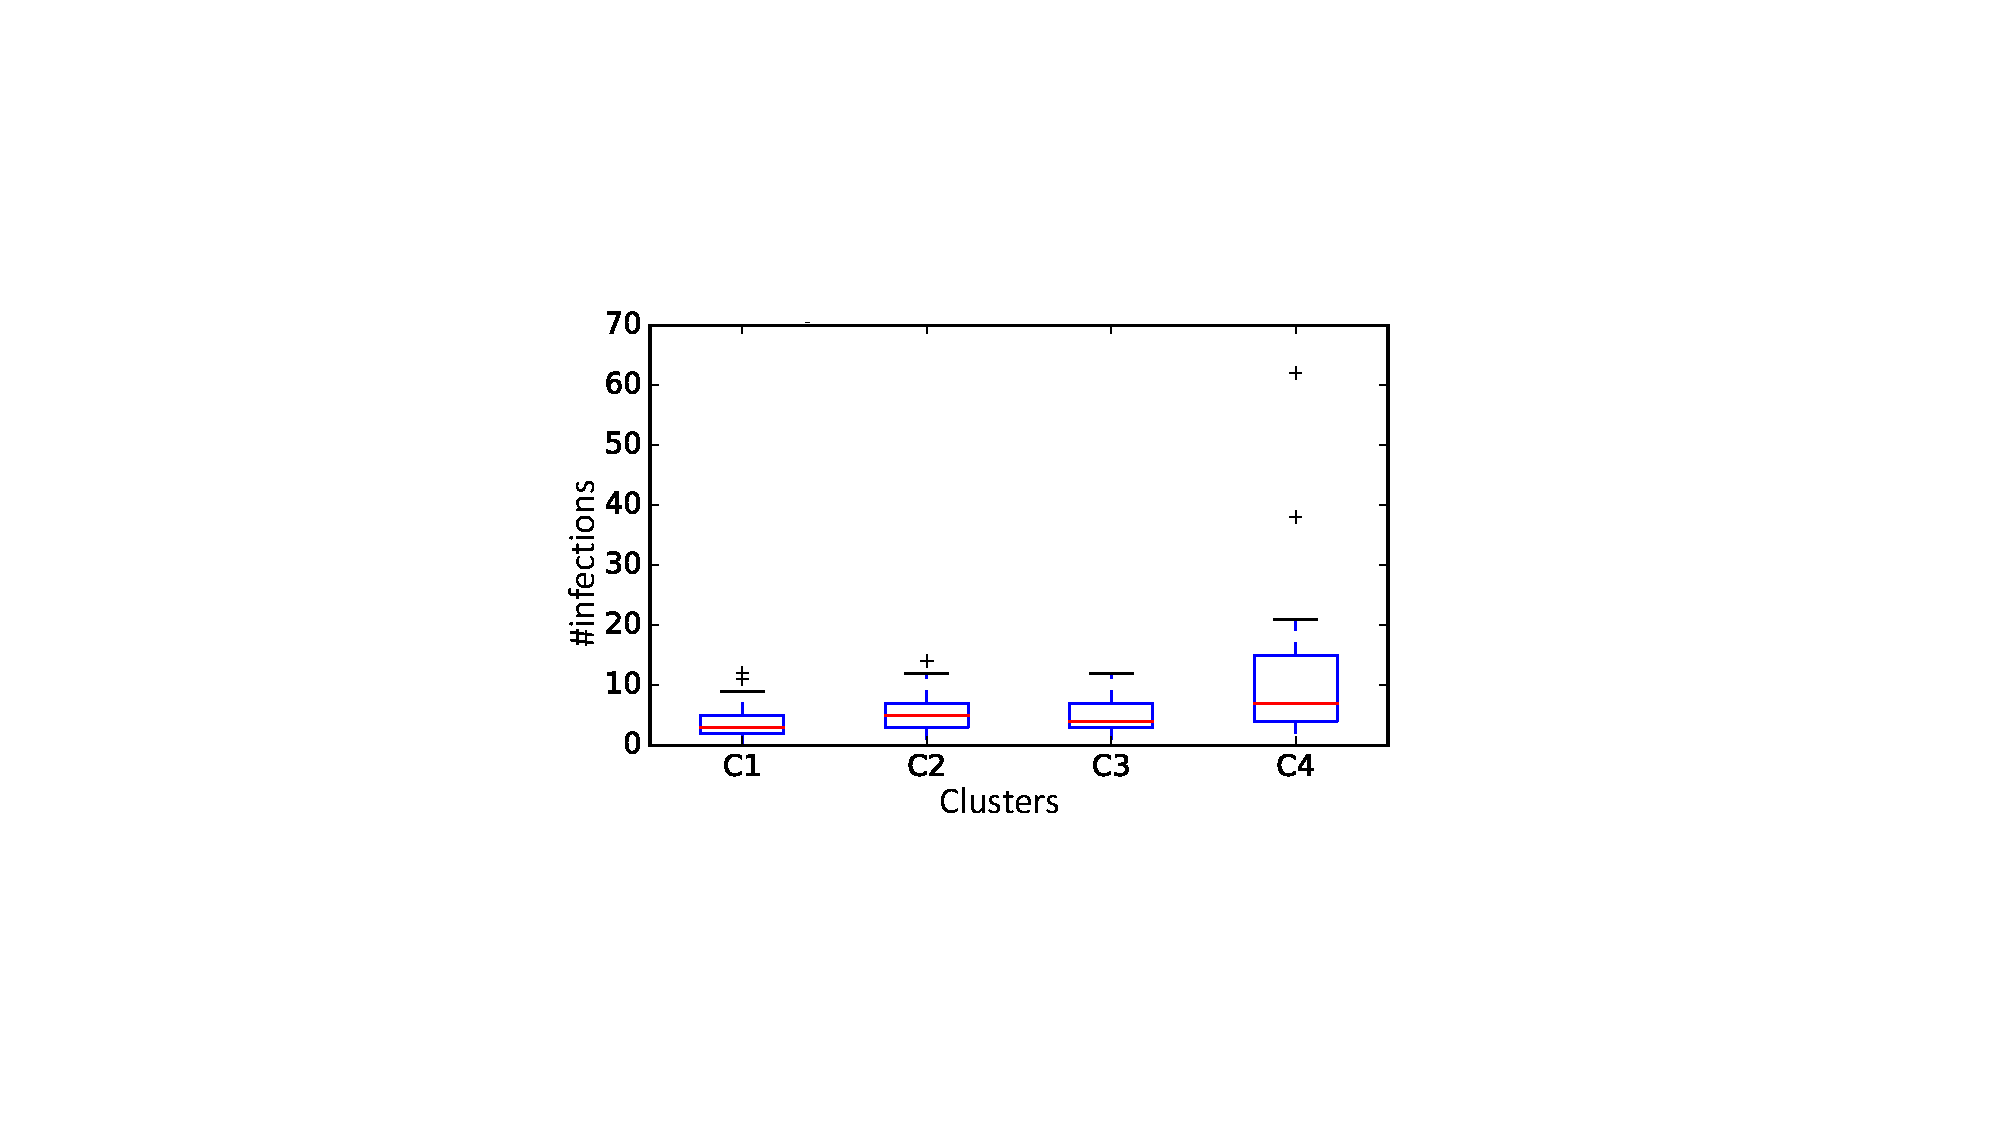
\includegraphics[width=.35\textwidth]{img/criticality-schools-mn.pdf}
\vspace{-.2in}
\caption{Comparison of the distributions of the number of infections resulting from an
outbreak starting in each of  four underimmunized clusters in MN identified in \cite{cadena:vacc-cluster}.}
\label{fig:criticality-compare}
\end{figure}

We compute the criticality of the four most significant underimmunized clusters in MN, as identified in \cite{cadena:vacc-cluster}.
The clusters are numbered 1--4 based on their significance, with respect to
underimmunization rates, so that cluster 1 is more significant than cluster 4.
However, as shown in Figure \ref{fig:criticality-compare},
\emph{it seems clear that the outbreak-size of cluster 4 is much higher than
that of cluster 1}---the 95th percentile value for the number of infections in
cluster 4 is almost four times that of cluster 1.
This implies criticality is not directly correlated with the level of underimmunization.

\subsection{Optimization power}
\label{sec:opt-power}
In Figure \ref{fig:cri-baseline-compare}, we show the criticality obtained by \algomaxcrit{} compared to the three baseline methods as a function of $k$. As expected, selecting subgraphs at random performs poorly and results in almost no additional infections compared to the initial disease conditions. Surprisingly, \textsc{Vulnerability} does not perform much better than \textsc{Random}. It is also interesting that the population-based heuristic does not have monotonic improvement with $k$. Even though the subgraph of size 9 has 55,800 inhabitants, the smaller subgraph of size 5 with a population of 34,000 leads to a much larger outbreak. 
Overall, the \textsc{Population} heuristic has better performance among the baselines, and it even surpasses our algorithm for $k=5$. However, \algomaxcrit{} exhibits notably better performance in general. The maximum improvement on criticality occurs on the 9-node cluster, where our method finds a cluster that leads to 4 times more infections than the \textsc{Population} baseline.

\begin{figure}
\centering
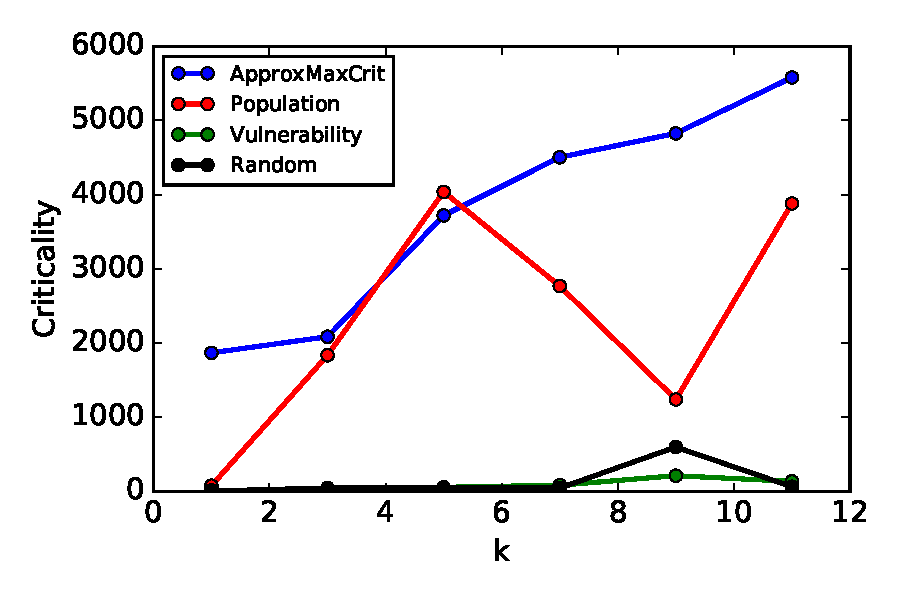
\includegraphics[width=.35\textwidth]{img/criticality-baseline-comparison.pdf}
\vspace{-.2in}
\caption{Comparison of algorithms for the \maxcrit{} problem as a function of the solution size $k$}
\label{fig:cri-baseline-compare}
\end{figure}

Another important quantity is the probability of having a large outbreak.
In Figure \ref{fig:crit-boxplots}, we show the distribution of criticality values 
for each method over 100 simulations of the disease model.
We observe that even the largest outbreaks caused by \textsc{Vulnerability} and \textsc{Random} are much smaller than those of \algomaxcrit{} and the \textsc{Population} baseline. We also note that the population-based clusters have larger variance in criticality and can result in larger outbreaks than those from our algorithm. This suggests that if the goal for a public health department is to prevent the worst-case scenario, then intervening the most-populated areas is a good heuristic. However, in doing so, one could miss smaller regions that, on average, are likely to infect more people.
%We report similar results on optimization power for \algoavgcrit{} in the Supplementary Material.

\begin{figure*}
\centering
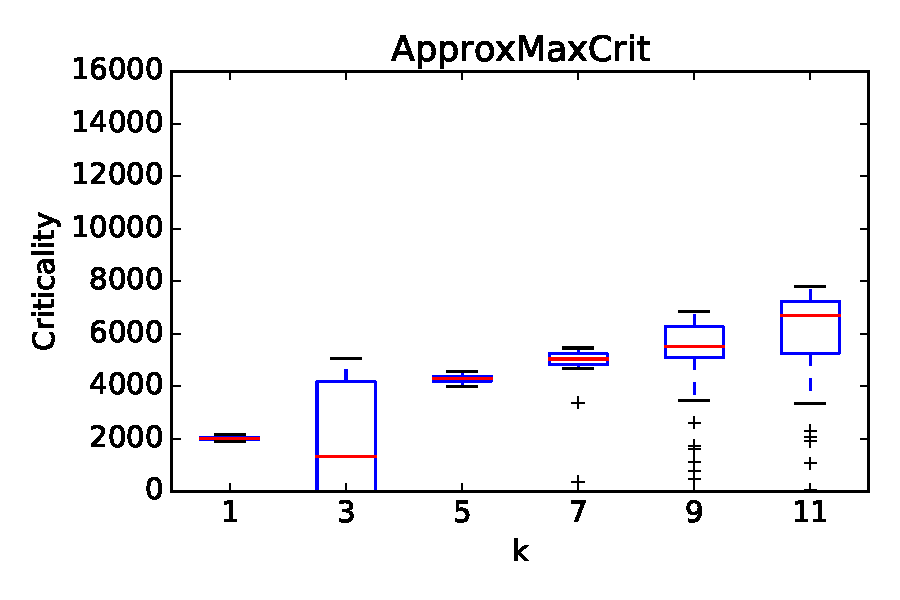
\includegraphics[width=0.24\textwidth]{img/mn_criticality_cluster_boxplot.pdf}
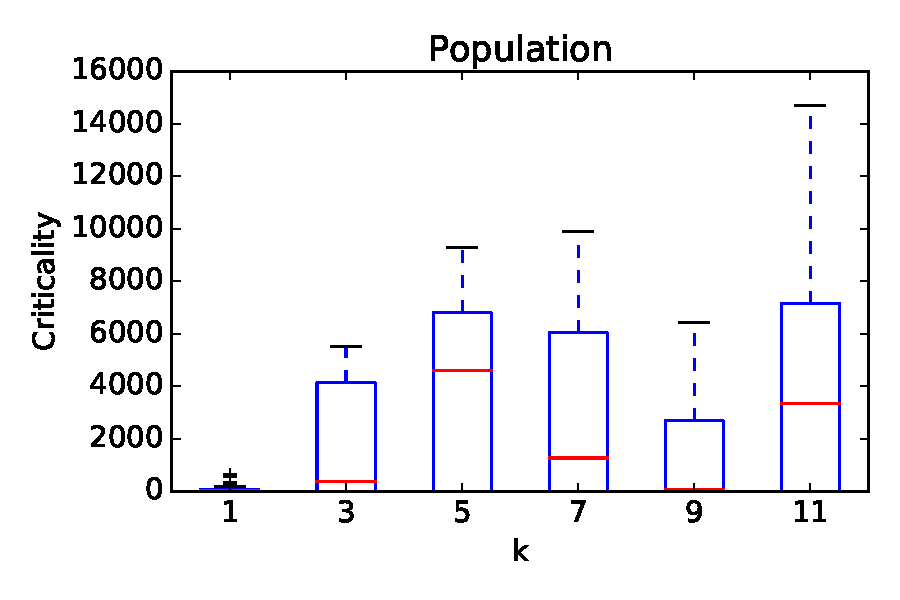
\includegraphics[width=0.24\textwidth]{img/mn_popsize_cluster_boxplot.pdf}
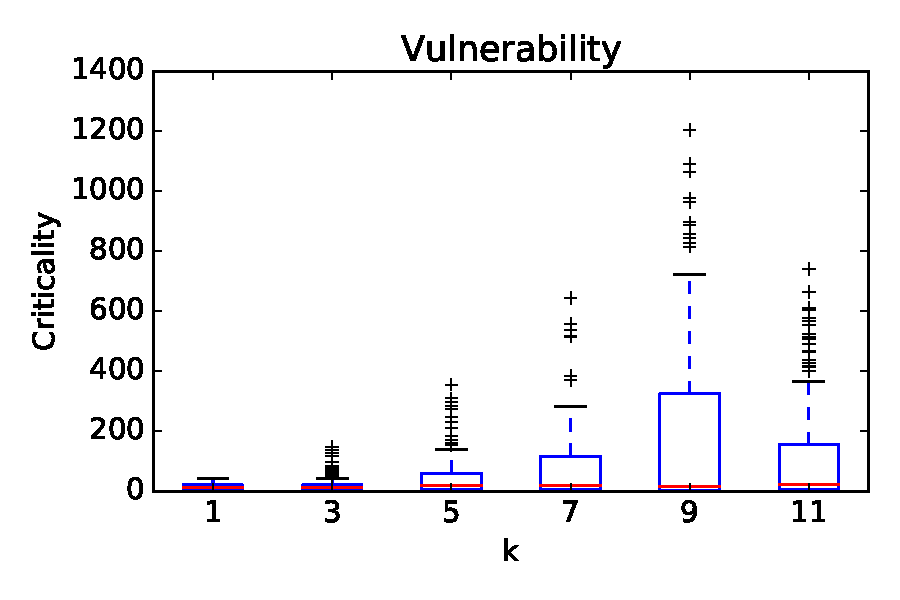
\includegraphics[width=0.24\textwidth]{img/mn_avg_blkgrp_cluster_boxplot.pdf}
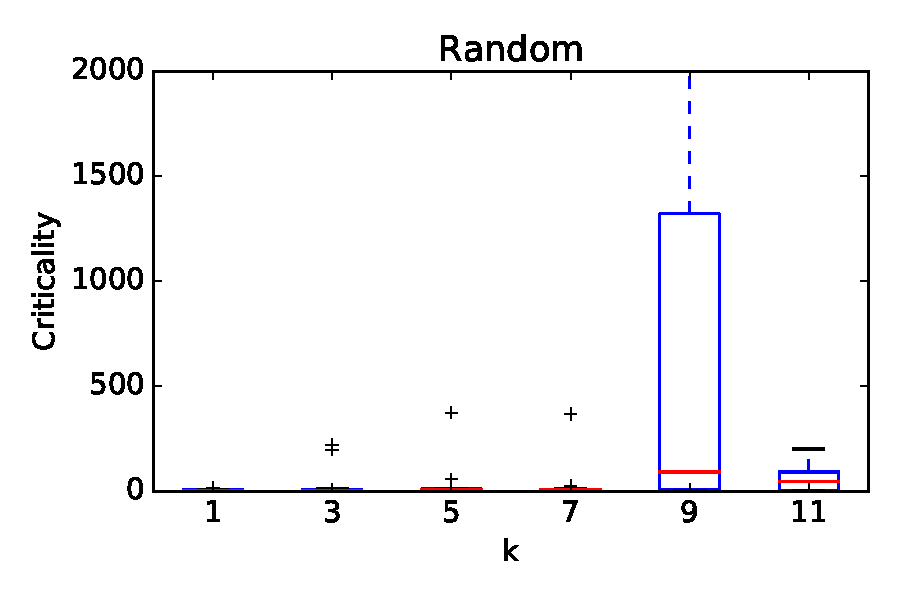
\includegraphics[width=0.24\textwidth]{img/mn_random_blkgrp_cluster_boxplot.pdf}\\
\caption{Criticality scores over 100 runs of the disease model for each method evaluated}
\label{fig:crit-boxplots}
\end{figure*}

\subsection{Critical clusters and demographics}
\label{sec:demographics}
We compare the distribution of age and income in the cluster discovered by \algomaxcrit{} ($k=11$) to that of the entire state. We aggregate household income into ``Low'' (below \$25,000), ``Medium'' (between \$25,000 and \$75,000), and ``High'' (above \$75,000). Ages are binned into ``Pre-school'' (below 5 years old), ``School'' (between 5 and 18 years old), ``Adult'' (between 18 and 70 years old), and ``Senior'' (above 70 years old). In Figure \ref{fig:cluster-demographics}, we see the critical cluster has significantly more households of low income compared to the entire state---19.6\% to 34.9\%. Similarly, children are over-represented. 26.6\% of the population are children in ``School'' age compared to the average of 18.7\%.

\begin{figure}
\centering
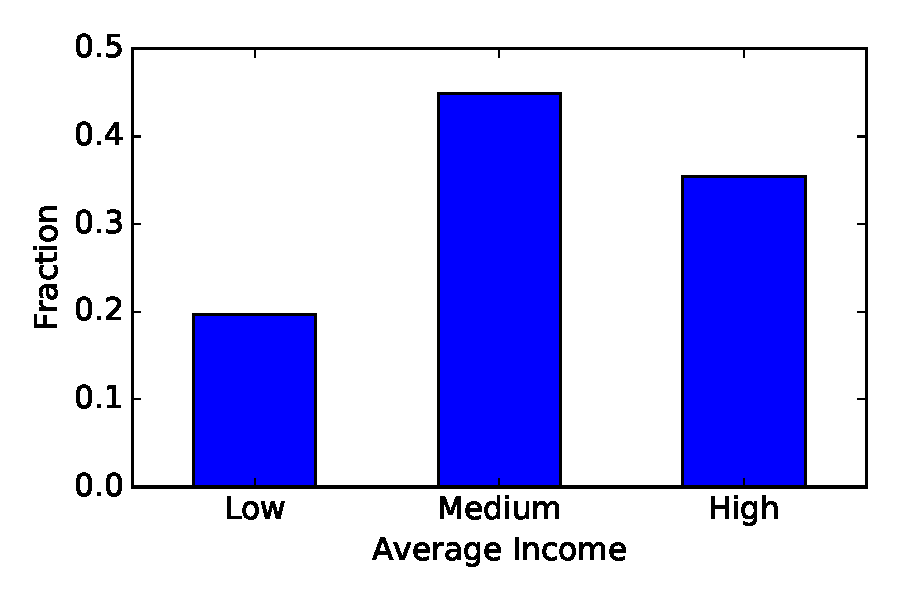
\includegraphics[width=0.23\textwidth]{img/mn-income.pdf}
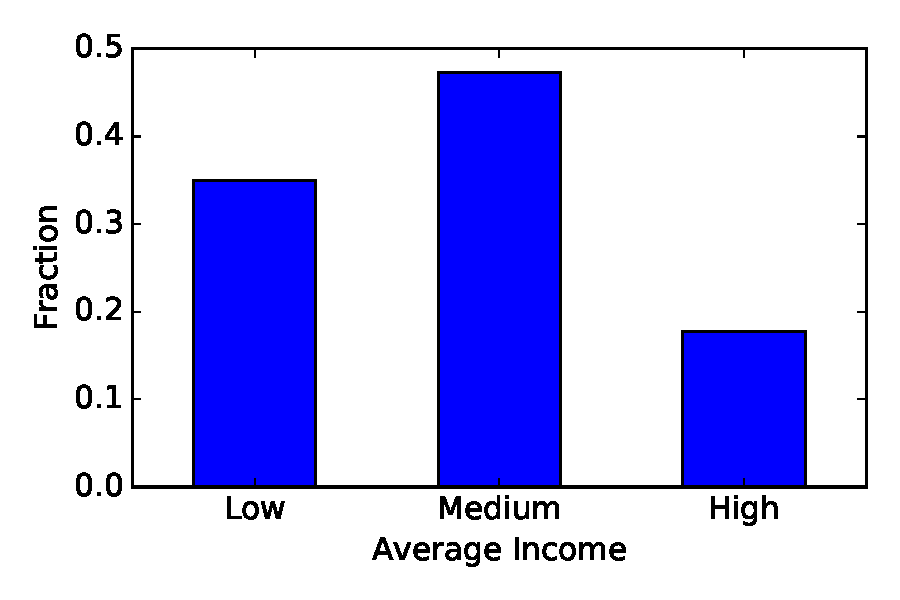
\includegraphics[width=0.23\textwidth]{img/kmaxst-11-income.pdf}
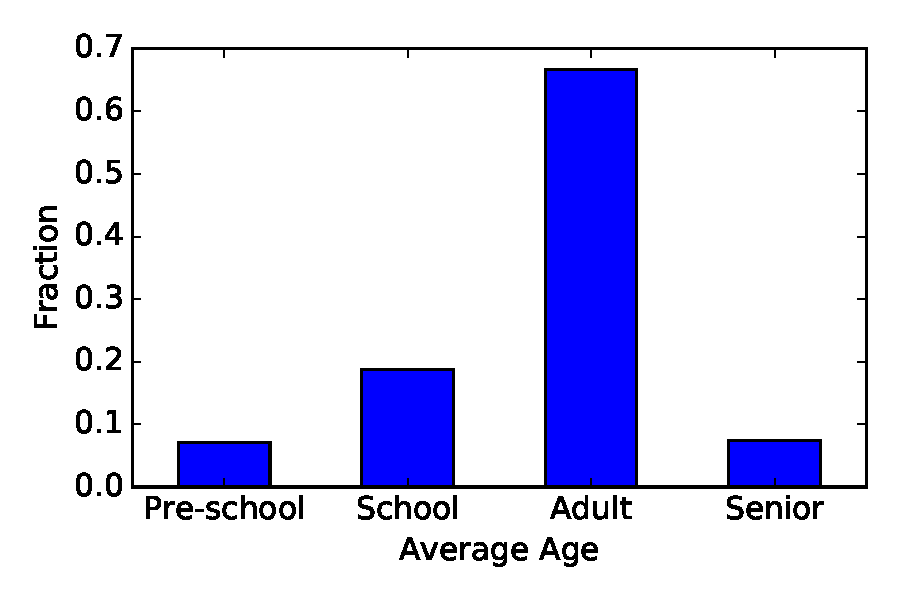
\includegraphics[width=0.23\textwidth]{img/mn-age.pdf}
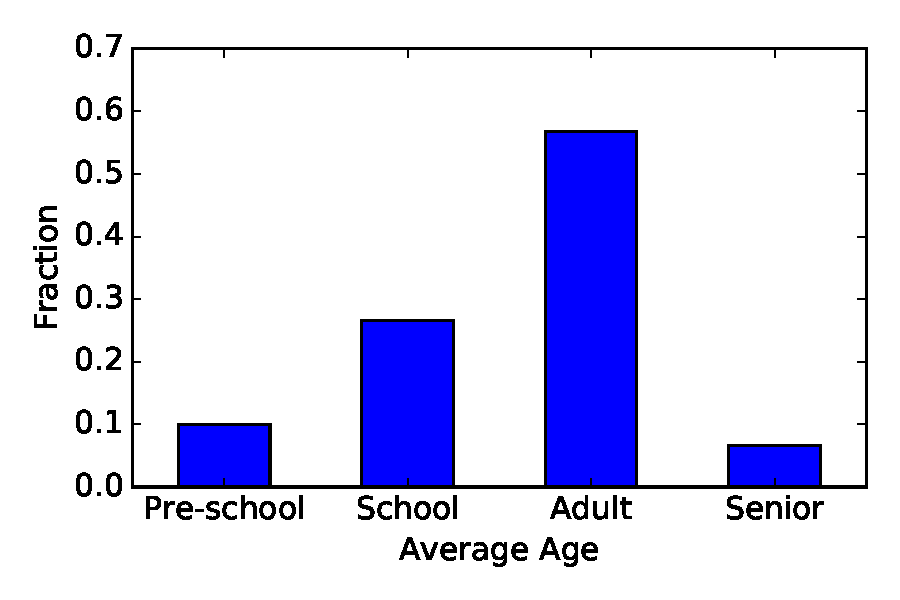
\includegraphics[width=0.23\textwidth]{img/kmaxst-11-age.pdf}
\caption{Average income (top) and age (bottom) in the entire state (left) and in the cluster discovered by \algomaxcrit{} (right). There are more children in school age and lower income households in the discovered critical cluster.}
\label{fig:cluster-demographics}
\end{figure}

We find critical clusters in different regions over Minnesota. Figure \ref{fig:mn-criticalsets} shows the top 10 non-overlapping clusters discovered using \algomaxcrit{}. The most critical cluster---with over 5,000 infections---is located on the rural northern part of the state, spanning the Leech Lake and Red Lake reservations. We note that this cluster results in the largest spread despite having a relatively small population of 14,910 people compared to clusters in urban regions. For example, the second most critical cluster---north of Minneapolis---has 48,889 inhabitants. %One possible explanation is that the largest cluster spans a larger geographical area, which could make the criticality function in that region closer to being modular than submodular. 

In addition to analyzing the most critical cluster, we look at the top-5 non-overlapping clusters discovered by \algomaxcrit{}. These correspond to different choices of root on the k-\textsc{MaxST} algorithm. In Table \ref{tab:top5-scores}, we report the total population size, criticality, and percentage of infections to the total population of the cluster---i.e., criticality / population. Note that this latter number could be larger than 1, since there are infections outside the cluster. As we discussed before, the top region leads to a large spread (41\% of its population size) despite having less inhabitants than the successive clusters. The second cluster has very similar criticality score, but in a more urban region.

\begin{table}
\centering
\caption{Total population and criticality in the top 5 clusters discovered by \algomaxcrit{}
%\vspace*{-.15in}
}
\label{tab:top5-scores}
\begin{tabular}{|c|r|r|r|}
\hline
\textbf{Rank} & \textbf{Population} & \textbf{Criticality} & \textbf{\% population}\\
\hline
1 & 14,910 & 6,138 & 41.2\%\\
2 & 48,889 & 6,093 & 12.5\%\\
3 & 23,391 & 1,388 & 5.9\%\\
4 & 15,731 &   647 & 4.1\%\\
5 &  9,936 &   372 & 4.7\%\\
\hline
\end{tabular}
\end{table}

Finally, we repeat our experiments for \maxcrit{} on the Minneapolis area instead of the entire state. The most critical cluster covers Brooklyn Park, where measles outbreaks occurred in 2017 and 2019\footnote{\url{https://tinyurl.com/y359zapv}}. However, we emphasize the need for domain-expert analysis to better interpret and make use of these results.
%, highlighted in red in Figure \ref{fig:brooklyn-park}, covers Brooklyn Park, where measles outbreaks occurred in 2017 and 2019\footnote{\url{https://tinyurl.com/y359zapv}}. However, we emphasize the need for domain-expert analysis to better interpret and make use of these results.

%\begin{figure}
%\centering
%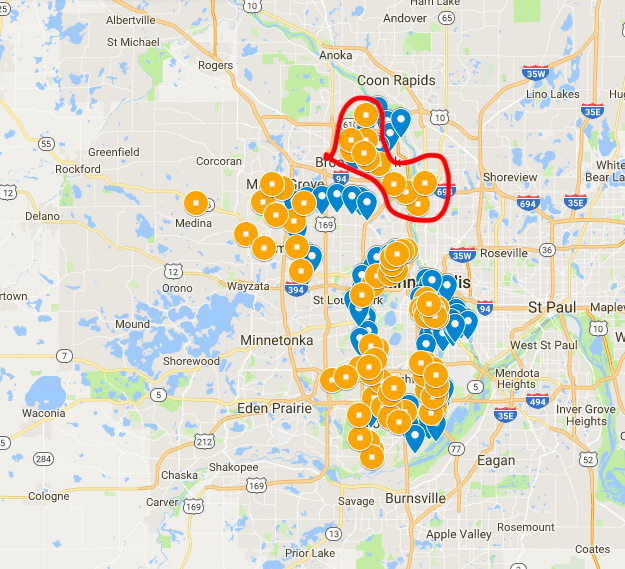
\includegraphics[width=0.4\textwidth]{img/maxcrit_minneapolis_clusters_higlighted.png}
%\caption{\maxcrit{} clusters in Minneapolis. Most critical cluster (highlighted in red) covers Brooklyn Park.}
%\label{fig:brooklyn-park}
%\end{figure}

%\begin{figure}
%\centering
%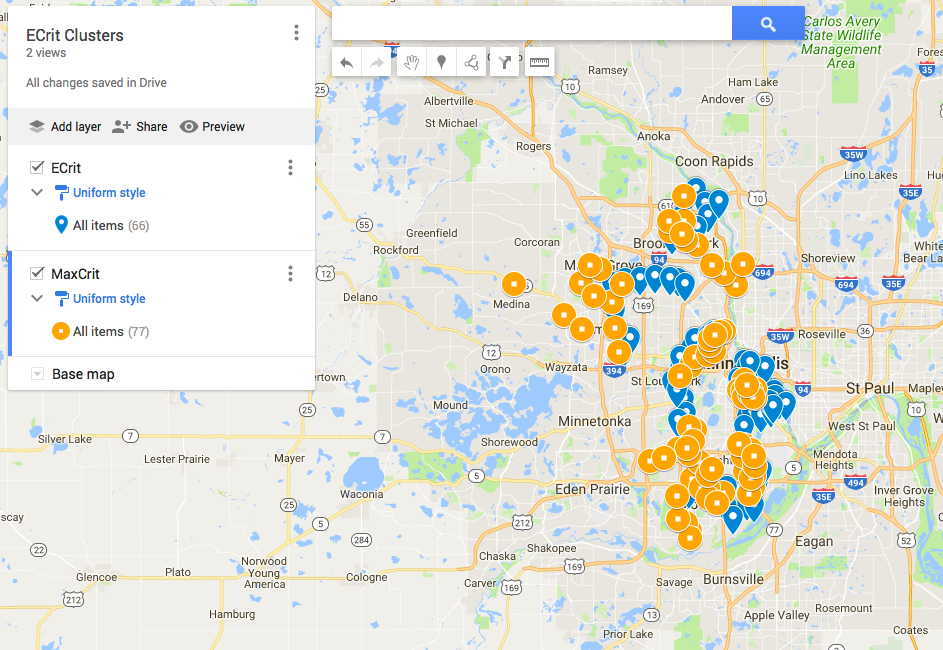
\includegraphics[width=0.4\textwidth]{img/maxcrit_minneapolis_clusters.png}
%\caption{\maxcrit{} and \avgcrit{} clusters in Minneapolis. Both solutions find similar critical clusters.}
%\label{fig:both-clusters}
%\end{figure}

%\subsection{\avgcrit}
%\begin{figure}
%\centering
%\includegraphics[width=.45\textwidth]{img/ecrit-baseline-comparison.pdf}
%\vspace{-.2in}
%\caption{Comparison of algorithms for \avgcrit{} as a function of the solution size $k$}
%\label{fig:ecrit-baseline-compare}
%\end{figure}


%\subsection{Criticality Based on Vulnerability}
%First, we study the criticality of the critical regions discovered by maximizing vulnerability. In Figure \ref{fig:cri-set-k12}, we observe the effect of leaving the most vulnerable region unvaccinated as a function of compliance in that region, for a region size of $k=12$. If the region is left unvaccinated, we observe a substantial outbreak. Even if the rest of the population is well-vaccinated (i.e., rates of 80\%, 90\%, and 95\%), the disease still affects tens of thousands of people, corresponding to at least 1\% of the population. In fact, we need at least 50\% compliance on the critical region to stop the disease from taking off.

%\begin{figure}
%\includegraphics[scale=.5]{img/vulnerable-ct-compliance-k12-rate.pdf}
%\includegraphics[scale=.5]{img/vulnerable-ct-compliance-k12-counts.pdf}
%\caption{If a subgraph with high vulnerability has low vaccination compliance (less than 50\%), we observe a substantial outbreak even if the rest of the population has high compliance (80\%, 90\%, and 95\%).}
%\label{fig:cri-set-k12}
%\end{figure}
%
%In Figure \ref{fig:cri-set-k3}, we observe a similar effect even for a critical set of only 3 census tracts ($k=3$).
%
%\begin{figure}
%\includegraphics[scale=.5]{img/vulnerable-ct-compliance-k3-rate.pdf}
%\includegraphics[scale=.5]{img/vulnerable-ct-compliance-k3-counts.pdf}
%\caption{Same as Figure \ref{fig:cri-set-k12} but for $k=3$. Even for a set of only 3 census tracts, we observe an outbreak on the order of $10^5$ infections when the critical set has low compliance.}
%\label{fig:cri-set-k3}
%\end{figure}

%\begin{figure}
%\centering
%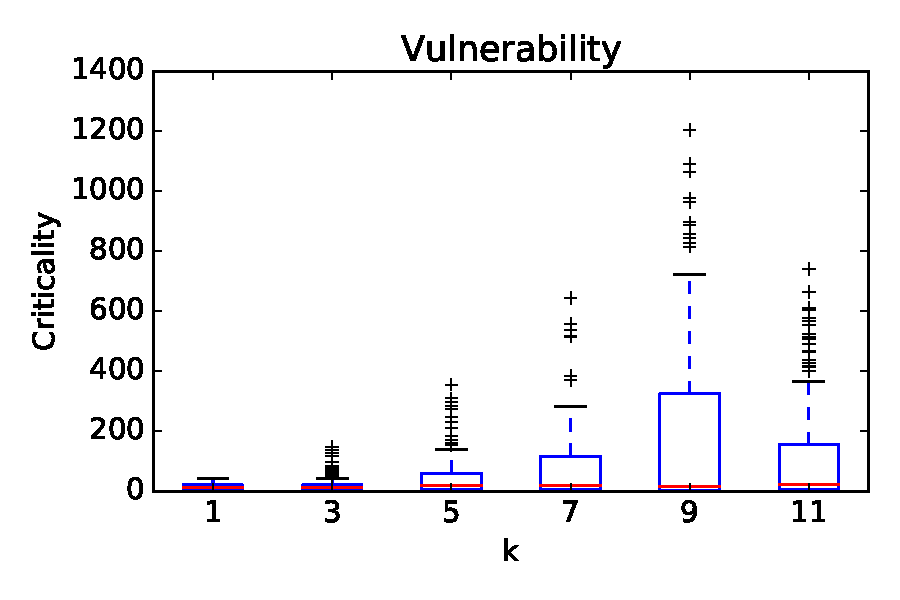
\includegraphics[scale=.5]{img/mn_avg_blkgrp_cluster_boxplot.pdf}	
%\includegraphics[scale=.5]{img/random-clusters-mn-blkgrp-boxplot.pdf}
%\caption{Distribution of criticality over multiple simulations.}
%\label{fig:cri-boxplots}
%\end{figure}
%
%
%\subsection{Comparison to random subgraphs.} In order to compare our algorithm based on maximizing vulnerability, we compare the graph that we found with 100 randomly sampled connected subgraphs. In Figure \ref{fig:cri-random}, we show the distribution of number of infections of this random subgraphs for a compliance rate of 95\% in the population outside the subgraph---left is for $k=12$ and right is for $k=3$. We find that our algorithm discovers a subgraph that is in the 99th percentile of this distribution; further, the subgraph that scores higher than our method has high overlap with the subgraph we discover. Thus, maximizing vulnerability is a strong heuristic for criticality.

%\begin{figure}
%\centering
%\includegraphics[scale=.5]{img/random-ct-compliance95-k12-counts.pdf}
%\includegraphics[scale=.5]{img/random-ct-compliance95-k3-counts.pdf}
%\caption{Distribution of attack rates in 100 random subgraphs of 12 (left) and 3 (right) random connected subgraphs. 99\% of the time maximizing modularity performs better.}
%\label{fig:cri-random}
%\end{figure}

%\subsection{Locations of Critical Regions}
%In Figure \ref{fig:critical-seattle}, we show the locations of the 10 regions with highest vulnerability in the Seattle dataset. Critical regions correspond to eithe 1) highly populated places, and 2) places with many children.
%
%\begin{figure}
%\centering
%\includegraphics[scale=.35]{img/critical-sets-k3-markers.png}
%\caption{Locations of the 10 subsets of size 3 with highest vulnerability. The stars mark the subset with highest vulnerability.}
%\label{fig:critical-seattle}
%\end{figure}

% !TEX root = ./main.tex
\section{Related Work}
Mathematical models have played an important role in epidemiology for over a century \cite{anderson+m:book}. Traditionally, epidemiological models have been differential equation models, which assume very simplistic mixing patterns of the underlying population. In the last decade, several research groups have developed agent based methods
using complex networks as a way to model more realistic mixing
\cite{eubank:nature04,longini05:science,fc+06,Liu2015}.
Such methods have been used for policy analysis
by local and national government agencies \cite{halloran:pnas08}.
We use this paradigm in our work.

All prior work on undervaccinated clusters has been restricted to identifying these clusters.
For instance, \cite{lieu2015geographic} analyze health records 
of children in Northern California to identify
significant clusters of under-immunization and vaccine refusal
using spatial scan statistics. However, such methods are not directly useful for the
question of identifying \emph{critical} clusters, which is our focus.

There is a large body of work related to outbreak detection in networks. \cite{christakis:10:sensor} use the ``friend of random people'' effect to monitor a subset of people and infer characteristics of the  epicurve for the entire population. \cite{Leskovec@KDD07} study early detection of different kinds of events---e.g., in water networks or social networks. However, these approaches have been focused on either just detecting that some event (e.g., start of an infection) has occurred or the epidemic characteristics for the entire region. Instead, we are interested in finding regions that would lead to a big number of infections if left unvaccinated.

Our work is also related to submodular function maximization with connectivity constraints. Connectivity makes the problem much more difficult than other constraints, such as cardinality or matroid constraints, which can be approximately optimized using a simple greedy procedure \cite{nemhauser1978analysis}. 
The most relevant work is by \cite{kuo2015maximizing}, who proposed a 
$\Omega(1/\sqrt{k})$ approximation algorithm to this problem. As mentioned earlier, our algorithm \algosubmod{} improves on this bound. Finally,
\cite{krause2006near} propose an approximation algorithm for budgeted 
submodularity maximization on graphs based on exploiting local structure. 


% !TEX root = ./main.tex
\section{Conclusions}

Prior research has identified geographical clusters of undervaccinated
populations in many states. However, the potential risk of causing large outbreaks from such clusters is not well understood, and is the motivation of our work. Public health response (e.g., surveillance and field work within such a cluster) is very costly, and therefore, a method to quantify such risk would be an important public health contribution.


We formalize the problem \maxcrit{}
for finding critical clusters for highly contagious diseases that can be prevented by vaccination. 
We design algorithm \algomaxcrit{} and prove a rigorous worst case approximation guarantee for it. Our main technical contribution is a new algorithm for maximizing a submodular function on a network with connectivity constraints, and our algorithm improves on the previous best result for this problem by exploiting the doubling dimension of the network.
Experimental results show that our method performs significantly better than heuristics from public health. Such an approach can help public health agencies prioritize response to the challenges of reduced vaccination coverage.




\clearpage
{\small
\bibliographystyle{ACM-Reference-Format}
\bibliography{msmsort}
}

\clearpage
% !TEX root = ./main.tex
\section*{Supplementary Material}

\section{Additional details for Section \ref{sec:problem-statement}}
\label{sec:problem-statement-app}
\noindent
\textbf{Influence Maximization.} In the Influence Maximization (\infmax) problem \cite{kempe:sigkdd03}, we are given a directed graph $G=(V,E)$ and edge weights $p(u, v) \in [0, 1]$ indicating the probability that node $u$ influences node $v$. The goal is to find a set $S \subset V$ of $k$ \emph{seed nodes} to infect, such that the expected number of influenced nodes or \emph{spread}, $\sigma(S)$, is maximized. A commonly-used diffusion process in the IM problem is the Independent Cascade model \cite{kempe:sigkdd03}, in which each recently-influenced node $u$ has one chance to influence each neighbor $v$, succeeding with probability $p(u,v)$.
Note that an instance of \infmax{} consists only of a contact graph $G$, whereas an instance of \maxcrit{} consists of the contact graph $G$, a partition of the nodes of $G$ into regions, $\R$, and an
auxiliary graph $H_{\R}$ that captures connectivity among $\R$.

\begin{theorem}
%\label{theorem:nphard}
\maxcrit{} is NP-hard. 
\end{theorem}

\begin{proof}
\infmax{} is polynomial-time reducible to \maxcrit{}, which implies the NP-hardness, since \infmax{} is NP-hard. We construct a suitable auxiliary graph $H_{\R}$ and a vaccination vector $\mathbf{x}$, showing that the spread from the Independent Cascade model in the instance of \infmax{} is stochastically equivalent to the SEIR process in the instance of \maxcrit{}.

Suppose we are given an arbitrary instance of IM; that is, a directed graph $G_\infmax=(V_\infmax,E_\infmax)$, edge probabilities $p(u,v)$ for every edge $e=(u,v) \in E$, and parameter $k$. We will create an instance of \maxcrit{} with social contact network $G_\maxcrit = (V_\maxcrit, E_\maxcrit)$, region graph $\HR$ transmission probabilities $p'(\cdot)$, intervention $\mathbf{x}$, and parameter $k'=k+1$.

\noindent
\textbf{To construct $G_\maxcrit{}$}, we first add all the nodes and edges from $G_\infmax$. We call these nodes \emph{original}. Then, for every node $v \in V_\infmax{}$, we add a \emph{switch} node $v'$ and directed edge $(v', v)$. Additionally, we add a \emph{source} node $\src$ and undirected (or bidirectional) edges from $\src$ to each switch node $v'$.
Then, $G_\maxcrit{}$ is a graph with node set $V_\maxcrit{} = V_\infmax{} \cup \{v'| v \in V_\infmax{}\} \cup \{\src\}$ and edge set $E_\maxcrit{} = E_\infmax{} \cup \{(\src,v'), (v', \src), (v', v)|\ v \in V_\infmax{}\}$. Obviously, this construction can be performed in polynomial time in $G_\infmax{}$.

\noindent
\textbf{To construct $\HR$}, we define a set of regions $\R = \{r_v | v \in V_\infmax{}\} \cup \{r_\src\}$. That is, we have one region for each original node, plus one region for the source node. The nodes $v$ and $v'$ in $G_\maxcrit{}$ are associated with a corresponding region in $\HR$: $\loc(v)=\loc(v') = r_v$, for each $v,v'\in V_\maxcrit{}$; similarly, $\loc(\src) = r_\src$. Then, we let the graph $\HR$ be a star with center $r_\src$.

\noindent
\textbf{For the transmission probabilities}, we let $p'(u, v) = p(u,v)$, for all $e=(u,v) \in E_\infmax{}$.
Every edge from $v'$ to $v$ infects $v$ with probability 1; that is, $p'(v',v) = 1$, for all original nodes $v$. Similarly, $p'(\src, v') = p'(v', \src) = 1$, for all switch nodes $v'$.

\noindent
\textbf{The intervention vector} $\mathbf{x}$ is defined as follows. 
First, all the original nodes are left unvaccinated: $x_v = 0$, for all $v$. Second, all the switch nodes are vaccinated with probability 1: $x_{v'} = 1$, for all $v'$. Lastly, the source node $\src$ is unvaccinated, i.e., $x_{\src}=0$. 

\noindent
\textbf{Correspondence between Independent Cascade and SEIR.} Now, let $S_\infmax{}$ be a set of $k$ seed nodes in the instance of IM, and let $S_\maxcrit{}= \{v' | v \in S_\infmax{}\}$ be a set containing the corresponding switch nodes in the instance of \maxcrit{} constructed above. Set these switch nodes to be unvaccinated, and consider an SEIR process on the graph $G_\maxcrit{}$ in which the infectious period is 1 time step and node $\src$ is the only node infected initially. At time $t=0$, the process starts at node $\src$; then, at $t=1$, all the nodes in $S_\maxcrit{}$ are infected deterministically, and at $t=2$, all the nodes in $S_\infmax{}$---and only the nodes in $S_\infmax{}$---are infected. From here on, the SEIR process in $G_\maxcrit{}$ is stochastically equivalent to the Independent Cascade model in $G_\infmax{}$. 

\noindent
\textbf{Equivalence between instances.} To complete the proof, we claim that an instance of $\infmax{}(G_\infmax{}, k)$ is equivalent to the instance $\maxcrit{}(G_\maxcrit{}, \HR, k + 1)$.
In particular, there exists a solution $S_\infmax{}$ with spread $\sigma(S_\infmax{})$ to the former problem if and only if there exists a solution $S_\maxcrit{}$ to the latter with criticality $\crit(S_\maxcrit{}) = \sigma(S_\infmax{}) + k + 1$. 

$\Rightarrow$ Starting with $S_\infmax{}$, let $S_\maxcrit{}= \{r_v | v \in S_\infmax{}\} \cup \{r_\src\}$ be the set of corresponding regions in $\HR$, plus the region of the source node. By construction, these regions are connected in $\HR$, and $S_\maxcrit{}$ has size $|S_\infmax{}| + 1 = k + 1$, so it is a valid solution to $\maxcrit$. Furthermore, by the equivalence between Independent Cascade and SEIR, we have that $\crit(S_\maxcrit{}) = \sigma(S_\infmax{}) + k + 1$, where the $(k + 1)$ additional infections correspond to the source and switch nodes.

$\Leftarrow$ Conversely, let $S_\maxcrit{}$ be a solution to $\maxcrit{}$, which is a set of $(k+1)$ connected regions in $\HR$. Because $\HR$ is a star with $r_\src$ as its center, the node $r_\src$ has to be in $S_\maxcrit{}$; otherwise, the solution wouldn't be connected. Now, let $S_\infmax{}= \{v | r_v \in S_\maxcrit{} \setminus \{r_\src\}\}$ be the set of corresponding nodes in $G_\infmax{}$. Because $r_\src$ is in $S_\maxcrit$ and, by construction of the social contact network $G_\maxcrit{}$, the source node and $k$ switch nodes are guaranteed to be infected. After that, the SEIR process in $G_\maxcrit{}$ is equivalent to the Independent Cascade model in $G_\infmax{}$, giving us the claimed $\crit(S_\maxcrit{}) = \sigma(S_\infmax{}) + k + 1$.

%Thus, any instance of Influence Maximization under the Independent Cascade model can be viewed as an instance of \kcsp{} for the SIR process; %This completes the proof.
\end{proof}

\subsection{Impact of connectivity requirement}
The connectivity constraint has a strong effect on the solution of \maxcrit{}.
A solution computed for \infmax{} using the greedy algorithm of \cite{kempe:sigkdd03} can be arbitrarily suboptimal for the problem we propose. Informally, this follows because in \infmax{}, it is better to choose
the set of seeds to be located far apart, so that their combined influence is maximized.

\begin{observation}
%\label{obs:infmax}
There exists a family of instances $(G, H_{\R}, k)$ for which the optimum solution
$S^*$ to \maxcrit{} satisfies
$\maxcrit(S^*) =O(\frac{1}{k}\infmax(\hat{S}))$, where $\hat{S}$ is the optimum
solution to the \infmax{} version for this instance, without any connectivity requirements.
\end{observation}

For example, consider a cycle graph, as in Figure \ref{fig:observation-app}. Every node has one outgoing neighbor (clockwise direction), and every node infects its neighbor with probability 1, unless the neighbor is a blue node, in which case the probability is 0, as denoted in the figure. There are $k=4$ spreader nodes (in blue) separated by paths of length $k+1$. Consider an instance of $\infmax{}$ with size constraint $k$, and the analogous instance of $\maxcrit{}$, where, for simplicity, we assume that $G = \HR$. The optimal solution to \infmax{} consists of the $k$ hub nodes, with objective value equals to the number of nodes in the graph, $k(k+1)$, since each hub is able to propagate the infection through all the white nodes until the next clockwise hub. In contrast, the solution to \maxcrit{} must be a connected set of nodes, so the best solution would consist of a hub and the next $k$ clockwise white nodes, for an objective value of $k + 1$.

\begin{figure}
    \centering
    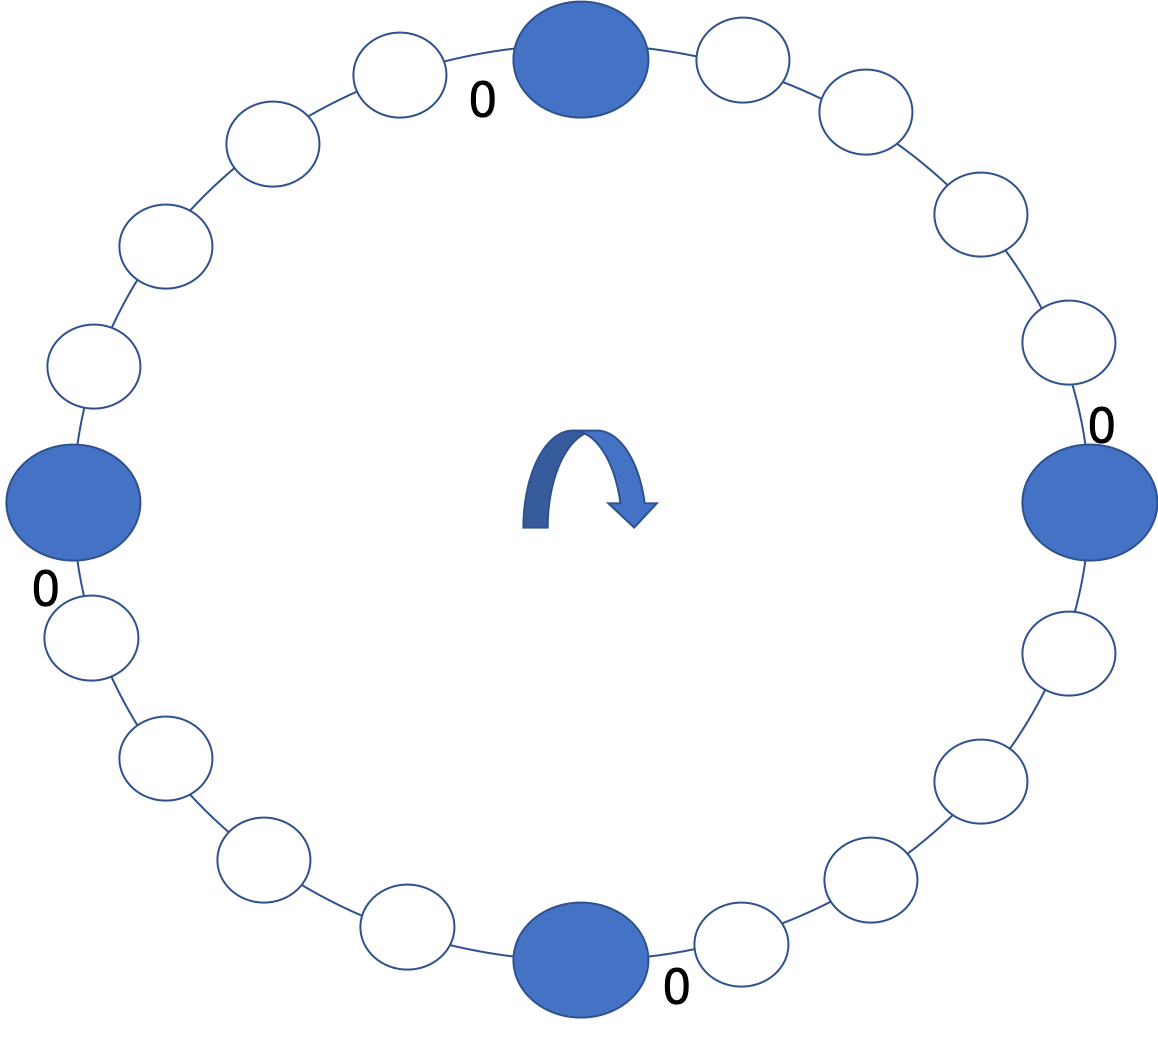
\includegraphics[width=.7\columnwidth]{img/observation.png}
    \caption{Effect of connectivity constraint in cycle graph with $k=4$ spreader nodes (blue) separated by paths of length $k + 1$. The optimal solution to $\infmax{}$ has $k$ times the objective value of the optimal solution for \maxcrit{}. See text for details.}
    \label{fig:observation-app}
\end{figure}

\section{Additional details for Section \ref{sec:proposed-critical}}
\begin{lemma}
Given a graph $G(V, E)$, $\crit(S)$ is a submodular function of $S \subset V$.
\end{lemma}

\begin{proof}
We follow the approach of Kempe et al.\ \cite{kempe:sigkdd03}, who analyze one random realization of the diffusion process at a time. For simplicity, we prove the submodularity of $\crit$ for the Independent Cascade model, but the result extends to the more general SEIR process. For each edge $e=(u,v)$, we flip a coin with bias equal to the transmission probability $p(u,v)$. Let $X(e)$ be a Bernoulli variable that is 1 with probability $p(u,v)$; then, we define the \emph{live} graph $L(V, E')$ as the subgraph of $G$ induced by the edges for which $X(e) = 1$: $L' = (V, E'=\{e \in E | X(e) = 1\})$. In the live graph, a node $v$ is infected by the end of the diffusion process if and only if $v$ is in the same component as one of the seeds in $S$. Without loss of generality, assume there is only one initial infection and let $r$ be the initially infected node. Then, the criticality of $S$ can be computed as
$$
\crit_L(S) = \left|\left(\bigcup_{s \in S} \text{comp}_L(s)\right) \cup \text{comp}_L(r)\right| - \left|\text{comp}_L(r)\right|.
$$
In words, the number of extra infections in $L$ due to node set $S$ is the size of the union of the components of nodes in $S$ minus the infections that we get if only $r$ is infected---i.e., the size of $\text{comp}_L(r)$.

Now, consider two sets $S,T$, such that $T\subseteq S$, and a node $v \not \in S$. The quantity $\crit_L(T \cup \{v\}) - \crit_L(T)$ is the number of extra infections from adding node $v$; that is, the number of elements in $\text{comp}_L(v)$ that are not already in $(\bigcup_{s \in T} \text{comp}_L(s)) \cup \text{comp}_L(r)$. This number is at least as large as the number of extra infections that we get by adding $v$ to the bigger set $S$, which gives us $\crit_L(T \cup \{v\}) - \crit_L(T) \geq \crit_L(S \cup \{v\}) - \crit_L(S)$. This is precisely the definition of submodularity, so the criticality function for a fixed live graph is submodular. Over random realizations of $L$, we obtain
$$
\crit(S) = \sum_{L}\text{Pr}(L) \crit_L(S).
$$
where $\text{Pr}(L)$ denotes the probability of obtaining the live graph $L$ with the edge probabilities $p(u,v)$. This is a convex combination of submodular functions, which is known to be submodular too, completing the proof.
\end{proof}

\subsection{Details on \greedy{} procedure and improving running time}
The $\greedy{}$ procedure in Algorithm \ref{alg:algosubmod} involves computing the criticality of every region in $\HR$ a number of times, which results in quadratic running time in the graph size. 
Instead, we use the efficient sampling approach of \cite{borgs:soda14} to significantly improve the running time. 
We call this faster procedure \textsc{FastGreedy} and show pseudocode in Algorithm \ref{alg:greedyborgs}. The inputs to \textsc{FastGreedy} are (1) the social contact network $G$, where the disease spreads, (2) a subset of regions $R\subset \R$, for which we want to find an approximate solution, (3) the vaccination vector when $R$ is undervaccinated, $\mathbf{x}^R$, and (4) the size constraint $k$. The algorithm returns a set $X \subset R$ of size $k$, just like the \greedy{} procedure. The main ideas are the following:
\begin{enumerate}
    \item We sample live graphs (defined in Section 8) until we observe at least $L=ck|E|\log{|V|}$ edges and store the components that are reachable from the source of the infection (lines 4--9)
    \item Then, we rank each node by the number of components it reaches (line 11)
    \item We form $X$ greedily by adding the $k$ nodes of highest rank, updating the ranking as we add nodes (lines 12--14) 
\end{enumerate}
As shown in \cite{borgs:soda14}, \textsc{FastGreedy} can be implemented to run in time $O(ck|E|\log{|V|})$.

\begin{algorithm}{}
\small
\caption{\small $\textsc{FastGreedy}(G=(V,E), R \subset \R, \mathbf{x}^R, k)$}
\label{alg:greedyborgs}
\begin{algorithmic}[1]
\STATE Let $\mathcal{S}=\emptyset$
\STATE Let $L=ck|E|\log{|V|}$, for a constant $c$
\STATE $\ell=0$
\WHILE{$\ell <L$}
  \STATE Pick random subgraph $G'$ of $G$ with (1) edges sampled based on
disease transmission probability, (2) nodes sampled with probability $1 - \mathbf{x}^R$
  \STATE $\ell = \ell + |E(G')|$
  \STATE Let $C_i$ be the set of components reachable from the set $\src_R$
of sources in $G'$
  \STATE $\mathcal{S} = \mathcal{S}\cup\{C_i\}$
\ENDWHILE
\STATE Initialize $X=\emptyset$
\STATE
For each $r\in R$, define $deg(r, \mathcal{S})$ to be the number
of sets $C_i\in\mathcal{S}$ that contain some node in $V(r)$
\FOR{$i=1$ to $k$}
  \STATE Append $r=\text{argmax}_{r'} deg(r',\mathcal{S})$ to $X$
\STATE
Remove all sets $C_i$ hit by $V(r)$ from $\mathcal{S}$ and update all $deg(\cdot)$
\ENDFOR
\STATE \textbf{return} $X$
\end{algorithmic}
\end{algorithm}


\begin{theorem}
\label{theorem:maxcrit-app}
If $\HR$ has doubling dimension $d$, algorithm  \algomaxcrit{} gives an $\Omega\Big(\frac{1}{k^{(d-1)/(2d-1)}}\Big)$ approximation to the \maxcrit{} problem, and it has worst case running time $O(ck^{\frac{d}{2d - 1}}|\R||E|\log{|V|} + |E_{\R}|(2e)^k)$.
\end{theorem}

\begin{proof}
The approximation guarantee follows from Theorem \ref{theorem:submod}. The running time is simply the sum of the running times of \algomaxst{} above and  \algosubmod{} implemented with \textsc{FastGreedy}. In \algosubmod{}, we invoke \textsc{FastGreedy} for each region in $\R$ using a size constraint of $\ell = k^{\frac{d}{2d - 1}}$, which gives us the claimed running time of $O(ck^{\frac{d}{2d - 1}}|\R||E|\log{|V|})$.
\end{proof}

\end{document}
